\documentclass[twoside]{book}

% Packages required by doxygen
\usepackage{fixltx2e}
\usepackage{calc}
\usepackage{doxygen}
\usepackage[export]{adjustbox} % also loads graphicx
\usepackage{graphicx}
\usepackage[utf8]{inputenc}
\usepackage{makeidx}
\usepackage{multicol}
\usepackage{multirow}
\PassOptionsToPackage{warn}{textcomp}
\usepackage{textcomp}
\usepackage[nointegrals]{wasysym}
\usepackage[table]{xcolor}

% Font selection
\usepackage[T1]{fontenc}
\usepackage[scaled=.90]{helvet}
\usepackage{courier}
\usepackage{amssymb}
\usepackage{sectsty}
\renewcommand{\familydefault}{\sfdefault}
\allsectionsfont{%
  \fontseries{bc}\selectfont%
  \color{darkgray}%
}
\renewcommand{\DoxyLabelFont}{%
  \fontseries{bc}\selectfont%
  \color{darkgray}%
}
\newcommand{\+}{\discretionary{\mbox{\scriptsize$\hookleftarrow$}}{}{}}

% Page & text layout
\usepackage{geometry}
\geometry{%
  a4paper,%
  top=2.5cm,%
  bottom=2.5cm,%
  left=2.5cm,%
  right=2.5cm%
}
\tolerance=750
\hfuzz=15pt
\hbadness=750
\setlength{\emergencystretch}{15pt}
\setlength{\parindent}{0cm}
\setlength{\parskip}{0.2cm}
\makeatletter
\renewcommand{\paragraph}{%
  \@startsection{paragraph}{4}{0ex}{-1.0ex}{1.0ex}{%
    \normalfont\normalsize\bfseries\SS@parafont%
  }%
}
\renewcommand{\subparagraph}{%
  \@startsection{subparagraph}{5}{0ex}{-1.0ex}{1.0ex}{%
    \normalfont\normalsize\bfseries\SS@subparafont%
  }%
}
\makeatother

% Headers & footers
\usepackage{fancyhdr}
\pagestyle{fancyplain}
\fancyhead[LE]{\fancyplain{}{\bfseries\thepage}}
\fancyhead[CE]{\fancyplain{}{}}
\fancyhead[RE]{\fancyplain{}{\bfseries\leftmark}}
\fancyhead[LO]{\fancyplain{}{\bfseries\rightmark}}
\fancyhead[CO]{\fancyplain{}{}}
\fancyhead[RO]{\fancyplain{}{\bfseries\thepage}}
\fancyfoot[LE]{\fancyplain{}{}}
\fancyfoot[CE]{\fancyplain{}{}}
\fancyfoot[RE]{\fancyplain{}{\bfseries\scriptsize Generated on Wed May 6 2015 03\+:36\+:10 for Zarzadzanie budynkami by Doxygen }}
\fancyfoot[LO]{\fancyplain{}{\bfseries\scriptsize Generated on Wed May 6 2015 03\+:36\+:10 for Zarzadzanie budynkami by Doxygen }}
\fancyfoot[CO]{\fancyplain{}{}}
\fancyfoot[RO]{\fancyplain{}{}}
\renewcommand{\footrulewidth}{0.4pt}
\renewcommand{\chaptermark}[1]{%
  \markboth{#1}{}%
}
\renewcommand{\sectionmark}[1]{%
  \markright{\thesection\ #1}%
}

% Indices & bibliography
\usepackage{natbib}
\usepackage[titles]{tocloft}
\setcounter{tocdepth}{3}
\setcounter{secnumdepth}{5}
\makeindex

% Hyperlinks (required, but should be loaded last)
\usepackage{ifpdf}
\ifpdf
  \usepackage[pdftex,pagebackref=true]{hyperref}
\else
  \usepackage[ps2pdf,pagebackref=true]{hyperref}
\fi
\hypersetup{%
  colorlinks=true,%
  linkcolor=blue,%
  citecolor=blue,%
  unicode%
}

% Custom commands
\newcommand{\clearemptydoublepage}{%
  \newpage{\pagestyle{empty}\cleardoublepage}%
}


%===== C O N T E N T S =====

\begin{document}

% Titlepage & ToC
\hypersetup{pageanchor=false,
             bookmarks=true,
             bookmarksnumbered=true,
             pdfencoding=unicode
            }
\pagenumbering{roman}
\begin{titlepage}
\vspace*{7cm}
\begin{center}%
{\Large Zarzadzanie budynkami \\[1ex]\large 1.\+0 }\\
\vspace*{1cm}
{\large Generated by Doxygen 1.8.9.1}\\
\vspace*{0.5cm}
{\small Wed May 6 2015 03:36:10}\\
\end{center}
\end{titlepage}
\clearemptydoublepage
\tableofcontents
\clearemptydoublepage
\pagenumbering{arabic}
\hypersetup{pageanchor=true}

%--- Begin generated contents ---
\chapter{Hierarchical Index}
\section{Class Hierarchy}
This inheritance list is sorted roughly, but not completely, alphabetically\+:\begin{DoxyCompactList}
\item \contentsline{section}{Budynek}{\pageref{class_budynek}}{}
\begin{DoxyCompactList}
\item \contentsline{section}{Sklep}{\pageref{class_sklep}}{}
\end{DoxyCompactList}
\item \contentsline{section}{Firma\+\_\+remontowa}{\pageref{class_firma__remontowa}}{}
\item \contentsline{section}{Obsluga\+\_\+podatkow}{\pageref{class_obsluga__podatkow}}{}
\item \contentsline{section}{Remiza}{\pageref{class_remiza}}{}
\item \contentsline{section}{Zarzadzanie\+\_\+budynkami}{\pageref{class_zarzadzanie__budynkami}}{}
\begin{DoxyCompactList}
\item \contentsline{section}{Zarzadanie\+\_\+wspoldzielnia}{\pageref{class_zarzadanie__wspoldzielnia}}{}
\begin{DoxyCompactList}
\item \contentsline{section}{Miejska}{\pageref{class_miejska}}{}
\item \contentsline{section}{Wiejska}{\pageref{class_wiejska}}{}
\end{DoxyCompactList}
\end{DoxyCompactList}
\end{DoxyCompactList}

\chapter{Class Index}
\section{Class List}
Here are the classes, structs, unions and interfaces with brief descriptions\+:\begin{DoxyCompactList}
\item\contentsline{section}{\hyperlink{class_budynek}{Budynek} \\*Klasa budynek }{\pageref{class_budynek}}{}
\item\contentsline{section}{\hyperlink{class_firma__remontowa}{Firma\+\_\+remontowa} \\*Klasa firmy remontowej }{\pageref{class_firma__remontowa}}{}
\item\contentsline{section}{\hyperlink{class_miejska}{Miejska} \\*Klasa miejska, dziedziczaca po klasie Zarzadzanie\+\_\+wspoldzielnia }{\pageref{class_miejska}}{}
\item\contentsline{section}{\hyperlink{class_obsluga__podatkow}{Obsluga\+\_\+podatkow} \\*Klasa umozliwiajaca obsluge podatkow }{\pageref{class_obsluga__podatkow}}{}
\item\contentsline{section}{\hyperlink{class_remiza}{Remiza} \\*Klasa symulujaca wiejska remize }{\pageref{class_remiza}}{}
\item\contentsline{section}{\hyperlink{class_sklep}{Sklep} \\*Klasa \hyperlink{class_sklep}{Sklep}, poszerzajaca mozliwosci Budynku o informacje o sklepie. Domyslnie jej rodzaj to 1 }{\pageref{class_sklep}}{}
\item\contentsline{section}{\hyperlink{class_wiejska}{Wiejska} \\*Klasa wiejska poszerze mozliwosci klasy bazowej o posiadanie \char`\"{}remizy\char`\"{} }{\pageref{class_wiejska}}{}
\item\contentsline{section}{\hyperlink{class_zarzadanie__wspoldzielnia}{Zarzadanie\+\_\+wspoldzielnia} \\*Klasa bazowa, projektu. Symuluje dzialanie Spoldzielni mieszkaniowej }{\pageref{class_zarzadanie__wspoldzielnia}}{}
\item\contentsline{section}{\hyperlink{class_zarzadzanie__budynkami}{Zarzadzanie\+\_\+budynkami} \\*Klasa abstrakcyjna }{\pageref{class_zarzadzanie__budynkami}}{}
\end{DoxyCompactList}

\chapter{Class Documentation}
\hypertarget{class_budynek}{}\section{Budynek Class Reference}
\label{class_budynek}\index{Budynek@{Budynek}}


Klasa budynek.  




{\ttfamily \#include $<$Budynek.\+h$>$}

Inheritance diagram for Budynek\+:\begin{figure}[H]
\begin{center}
\leavevmode
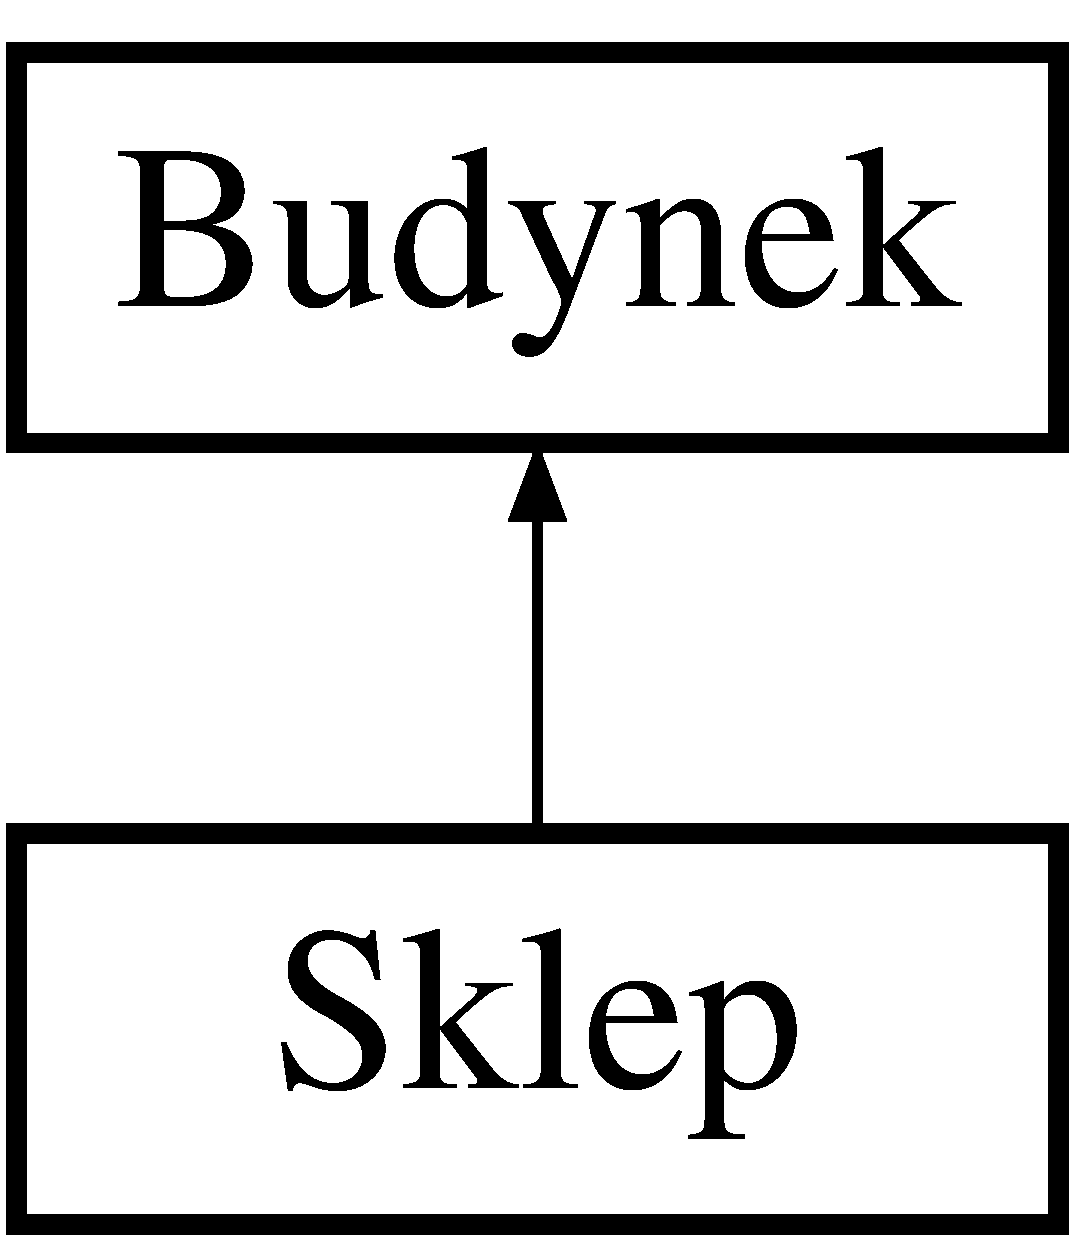
\includegraphics[height=2.000000cm]{class_budynek}
\end{center}
\end{figure}
\subsection*{Public Member Functions}
\begin{DoxyCompactItemize}
\item 
\hyperlink{class_budynek_a6130ff6245a4f097247c7f6ab68d14e2}{Budynek} (int r=0, char s=0)
\begin{DoxyCompactList}\small\item\em Konstruktor. \end{DoxyCompactList}\item 
\hypertarget{class_budynek_a6f682a6b4f44890413a20b87188dbcec}{}int \hyperlink{class_budynek_a6f682a6b4f44890413a20b87188dbcec}{zwroc\+Rodzaj} ()\label{class_budynek_a6f682a6b4f44890413a20b87188dbcec}

\begin{DoxyCompactList}\small\item\em -\/\+Funkcja zwracajaca rodzaj budynku. \end{DoxyCompactList}\item 
char \hyperlink{class_budynek_abba0db0edd3d93f17cb5132c60bbfaa2}{zwroc\+Stan} ()
\item 
\hypertarget{class_budynek_af5e0277c39c21e787f695ab93ed595e4}{}virtual void \hyperlink{class_budynek_af5e0277c39c21e787f695ab93ed595e4}{wczytaj\+\_\+z\+Pliku} (istream \&)\label{class_budynek_af5e0277c39c21e787f695ab93ed595e4}

\begin{DoxyCompactList}\small\item\em Funkcja umozliwiajaca wczytanie stanu obiektu z pliku. \end{DoxyCompactList}\item 
\hypertarget{class_budynek_a583785190d93363081f9c6c62d43cbdb}{}virtual void \hyperlink{class_budynek_a583785190d93363081f9c6c62d43cbdb}{zapisz\+\_\+do\+Pliku} (string)\label{class_budynek_a583785190d93363081f9c6c62d43cbdb}

\begin{DoxyCompactList}\small\item\em Funkcja umozliwiajaca zapisanie stanu obiektu do pliku. \end{DoxyCompactList}\item 
\hypertarget{class_budynek_abe365ed665adfe618be92e6767e628f3}{}void \hyperlink{class_budynek_abe365ed665adfe618be92e6767e628f3}{popraw\+Stan} (int)\label{class_budynek_abe365ed665adfe618be92e6767e628f3}

\begin{DoxyCompactList}\small\item\em Funkcja zwiekszenie stanu budynku. \end{DoxyCompactList}\end{DoxyCompactItemize}
\subsection*{Protected Attributes}
\begin{DoxyCompactItemize}
\item 
int \hyperlink{class_budynek_a99ad6ea24ed1e4d9acbe2855142de9b0}{rodzaj}
\item 
char \hyperlink{class_budynek_a790ff1e35e2c213152c6436fbb6ee285}{stan}
\end{DoxyCompactItemize}
\subsection*{Friends}
\begin{DoxyCompactItemize}
\item 
\hypertarget{class_budynek_a8e6044eb13005ebfaf1787db6fc51f59}{}ostream \& \hyperlink{class_budynek_a8e6044eb13005ebfaf1787db6fc51f59}{operator$<$$<$} (ostream \&, \hyperlink{class_budynek}{Budynek} \&)\label{class_budynek_a8e6044eb13005ebfaf1787db6fc51f59}

\begin{DoxyCompactList}\small\item\em Operator strumieniowy. \end{DoxyCompactList}\item 
\hypertarget{class_budynek_a8ad34897c6d555d7818558e38ef191c9}{}istream \& \hyperlink{class_budynek_a8ad34897c6d555d7818558e38ef191c9}{operator$>$$>$} (istream \&, \hyperlink{class_budynek}{Budynek} \&)\label{class_budynek_a8ad34897c6d555d7818558e38ef191c9}

\begin{DoxyCompactList}\small\item\em Operator strumieniowy. \end{DoxyCompactList}\end{DoxyCompactItemize}


\subsection{Detailed Description}
Klasa budynek. 

Klasa Umozliwiajaca tworzenie budynkow oraz zarzadzania nimi. 

\subsection{Constructor \& Destructor Documentation}
\hypertarget{class_budynek_a6130ff6245a4f097247c7f6ab68d14e2}{}\index{Budynek@{Budynek}!Budynek@{Budynek}}
\index{Budynek@{Budynek}!Budynek@{Budynek}}
\subsubsection[{Budynek(int r=0, char s=0)}]{\setlength{\rightskip}{0pt plus 5cm}Budynek\+::\+Budynek (
\begin{DoxyParamCaption}
\item[{int}]{r = {\ttfamily 0}, }
\item[{char}]{s = {\ttfamily 0}}
\end{DoxyParamCaption}
)}\label{class_budynek_a6130ff6245a4f097247c7f6ab68d14e2}


Konstruktor. 

Umozliwia stworzenie obiektu z okreslonym stanem poczatkowym. r-\/rodzaj, s-\/stan. 

\subsection{Member Function Documentation}
\hypertarget{class_budynek_abba0db0edd3d93f17cb5132c60bbfaa2}{}\index{Budynek@{Budynek}!zwroc\+Stan@{zwroc\+Stan}}
\index{zwroc\+Stan@{zwroc\+Stan}!Budynek@{Budynek}}
\subsubsection[{zwroc\+Stan()}]{\setlength{\rightskip}{0pt plus 5cm}char Budynek\+::zwroc\+Stan (
\begin{DoxyParamCaption}
{}
\end{DoxyParamCaption}
)}\label{class_budynek_abba0db0edd3d93f17cb5132c60bbfaa2}
-\/\+Funkcja zwracajaca stan budynku. 

\subsection{Member Data Documentation}
\hypertarget{class_budynek_a99ad6ea24ed1e4d9acbe2855142de9b0}{}\index{Budynek@{Budynek}!rodzaj@{rodzaj}}
\index{rodzaj@{rodzaj}!Budynek@{Budynek}}
\subsubsection[{rodzaj}]{\setlength{\rightskip}{0pt plus 5cm}int Budynek\+::rodzaj\hspace{0.3cm}{\ttfamily [protected]}}\label{class_budynek_a99ad6ea24ed1e4d9acbe2855142de9b0}

\begin{DoxyItemize}
\item Zmienna okreslajaca rodzaj budynku. (1.\+Dom; 2.\+Szeregowiec; 3.\+Budynek; 4.\+Wiezowiec) 
\end{DoxyItemize}\hypertarget{class_budynek_a790ff1e35e2c213152c6436fbb6ee285}{}\index{Budynek@{Budynek}!stan@{stan}}
\index{stan@{stan}!Budynek@{Budynek}}
\subsubsection[{stan}]{\setlength{\rightskip}{0pt plus 5cm}char Budynek\+::stan\hspace{0.3cm}{\ttfamily [protected]}}\label{class_budynek_a790ff1e35e2c213152c6436fbb6ee285}

\begin{DoxyItemize}
\item Zmienna Okreslajaca stan budynku w skali od 1 do 10. 
\end{DoxyItemize}

The documentation for this class was generated from the following file\+:\begin{DoxyCompactItemize}
\item 
/home/kamil/\+Pulpit/\+Elka/\+P\+R\+O\+E/\+P\+R\+O\+E-\/2/include/Budynek.\+h\end{DoxyCompactItemize}

\hypertarget{class_firma__remontowa}{}\section{Firma\+\_\+remontowa Class Reference}
\label{class_firma__remontowa}\index{Firma\+\_\+remontowa@{Firma\+\_\+remontowa}}


Klasa firmy remontowej.  




{\ttfamily \#include $<$Firma\+\_\+remontowa.\+h$>$}

\subsection*{Public Member Functions}
\begin{DoxyCompactItemize}
\item 
\hypertarget{class_firma__remontowa_a86d679b734a66ee5ffdd15f470815792}{}\hyperlink{class_firma__remontowa_a86d679b734a66ee5ffdd15f470815792}{Firma\+\_\+remontowa} ()\label{class_firma__remontowa_a86d679b734a66ee5ffdd15f470815792}

\begin{DoxyCompactList}\small\item\em Konstruktor domysly. \end{DoxyCompactList}\item 
int \hyperlink{class_firma__remontowa_acc5540b46df2bd85c4357870b2b086f5}{zwroc\+\_\+cene} (int)
\begin{DoxyCompactList}\small\item\em Funkcja zwracajaca cene rodzaju budynku. \end{DoxyCompactList}\item 
string \hyperlink{class_firma__remontowa_ac58421192dc9b68dcd5f7ed35faf58da}{zwroc\+\_\+nazwe} ()
\begin{DoxyCompactList}\small\item\em Funkcja zwracajaca nazwe firmy remontowej. \end{DoxyCompactList}\item 
\hypertarget{class_firma__remontowa_acd19620a53800f84df0fbe377f28dd64}{}void \hyperlink{class_firma__remontowa_acd19620a53800f84df0fbe377f28dd64}{info\+\_\+firma} ()\label{class_firma__remontowa_acd19620a53800f84df0fbe377f28dd64}

\begin{DoxyCompactList}\small\item\em Funkcja wyswietlajaca informacje o firmie. \end{DoxyCompactList}\item 
\hypertarget{class_firma__remontowa_a2097892c4af1ca175b73072d7b4176a7}{}void \hyperlink{class_firma__remontowa_a2097892c4af1ca175b73072d7b4176a7}{zmien\+\_\+nazwe} (string \&)\label{class_firma__remontowa_a2097892c4af1ca175b73072d7b4176a7}

\begin{DoxyCompactList}\small\item\em Funkcja umozliwiajaca zmiane nazwy firmy. \end{DoxyCompactList}\item 
void \hyperlink{class_firma__remontowa_a231e8446931c11fc608b5026204de56f}{zmien\+\_\+cene} (int, int)
\begin{DoxyCompactList}\small\item\em Funkcja umozliwiajaca zmiane ceny uslugi. \end{DoxyCompactList}\item 
\hypertarget{class_firma__remontowa_a0d15798ca03b0ebe81f333e25ee6c209}{}void \hyperlink{class_firma__remontowa_a0d15798ca03b0ebe81f333e25ee6c209}{wczytaj\+\_\+z\+Pliku} (istream \&)\label{class_firma__remontowa_a0d15798ca03b0ebe81f333e25ee6c209}

\begin{DoxyCompactList}\small\item\em Funkcja umozliwiajaca wczytanie stanu obiektu z pliku. \end{DoxyCompactList}\item 
\hypertarget{class_firma__remontowa_a982872b417e2d0dc7a44f95fcd05a3a5}{}void \hyperlink{class_firma__remontowa_a982872b417e2d0dc7a44f95fcd05a3a5}{zapisz\+\_\+do\+Pliku} (string)\label{class_firma__remontowa_a982872b417e2d0dc7a44f95fcd05a3a5}

\begin{DoxyCompactList}\small\item\em Funkcja umozliwiajaca zapisanie stanu obiektu do pliku. \end{DoxyCompactList}\end{DoxyCompactItemize}
\subsection*{Friends}
\begin{DoxyCompactItemize}
\item 
\hypertarget{class_firma__remontowa_ac3b1f713f74aaecd01167600c9166b25}{}ostream \& \hyperlink{class_firma__remontowa_ac3b1f713f74aaecd01167600c9166b25}{operator$<$$<$} (ostream \&, \hyperlink{class_firma__remontowa}{Firma\+\_\+remontowa} \&)\label{class_firma__remontowa_ac3b1f713f74aaecd01167600c9166b25}

\begin{DoxyCompactList}\small\item\em Operator strumieniowy. \end{DoxyCompactList}\item 
\hypertarget{class_firma__remontowa_a47a7efe31fd7ca3e995d2544635d252c}{}istream \& \hyperlink{class_firma__remontowa_a47a7efe31fd7ca3e995d2544635d252c}{operator$>$$>$} (istream \&, \hyperlink{class_firma__remontowa}{Firma\+\_\+remontowa} \&)\label{class_firma__remontowa_a47a7efe31fd7ca3e995d2544635d252c}

\begin{DoxyCompactList}\small\item\em Operator strumieniowy. \end{DoxyCompactList}\end{DoxyCompactItemize}


\subsection{Detailed Description}
Klasa firmy remontowej. 

Klasa umozliwia przeprowadzanie remontow budynkow w wspoldzielni. 

\subsection{Member Function Documentation}
\hypertarget{class_firma__remontowa_a231e8446931c11fc608b5026204de56f}{}\index{Firma\+\_\+remontowa@{Firma\+\_\+remontowa}!zmien\+\_\+cene@{zmien\+\_\+cene}}
\index{zmien\+\_\+cene@{zmien\+\_\+cene}!Firma\+\_\+remontowa@{Firma\+\_\+remontowa}}
\subsubsection[{zmien\+\_\+cene(int, int)}]{\setlength{\rightskip}{0pt plus 5cm}void Firma\+\_\+remontowa\+::zmien\+\_\+cene (
\begin{DoxyParamCaption}
\item[{int}]{, }
\item[{int}]{}
\end{DoxyParamCaption}
)}\label{class_firma__remontowa_a231e8446931c11fc608b5026204de56f}


Funkcja umozliwiajaca zmiane ceny uslugi. 


\begin{DoxyParams}{Parameters}
{\em pierwszy} & argument okresla rodzaj budynku, drugi nowa cene uslugi. \\
\hline
\end{DoxyParams}
\hypertarget{class_firma__remontowa_acc5540b46df2bd85c4357870b2b086f5}{}\index{Firma\+\_\+remontowa@{Firma\+\_\+remontowa}!zwroc\+\_\+cene@{zwroc\+\_\+cene}}
\index{zwroc\+\_\+cene@{zwroc\+\_\+cene}!Firma\+\_\+remontowa@{Firma\+\_\+remontowa}}
\subsubsection[{zwroc\+\_\+cene(int)}]{\setlength{\rightskip}{0pt plus 5cm}int Firma\+\_\+remontowa\+::zwroc\+\_\+cene (
\begin{DoxyParamCaption}
\item[{int}]{}
\end{DoxyParamCaption}
)}\label{class_firma__remontowa_acc5540b46df2bd85c4357870b2b086f5}


Funkcja zwracajaca cene rodzaju budynku. 


\begin{DoxyParams}{Parameters}
{\em rodzaj} & budynku. 1.\+Dom; 2.\+Szeregowiec; 3.\+Budynek; 4.\+Wiezowiec \\
\hline
\end{DoxyParams}
\begin{DoxyReturn}{Returns}
Zwraca cene uslugi. 
\end{DoxyReturn}
\hypertarget{class_firma__remontowa_ac58421192dc9b68dcd5f7ed35faf58da}{}\index{Firma\+\_\+remontowa@{Firma\+\_\+remontowa}!zwroc\+\_\+nazwe@{zwroc\+\_\+nazwe}}
\index{zwroc\+\_\+nazwe@{zwroc\+\_\+nazwe}!Firma\+\_\+remontowa@{Firma\+\_\+remontowa}}
\subsubsection[{zwroc\+\_\+nazwe()}]{\setlength{\rightskip}{0pt plus 5cm}string Firma\+\_\+remontowa\+::zwroc\+\_\+nazwe (
\begin{DoxyParamCaption}
{}
\end{DoxyParamCaption}
)}\label{class_firma__remontowa_ac58421192dc9b68dcd5f7ed35faf58da}


Funkcja zwracajaca nazwe firmy remontowej. 

\begin{DoxyReturn}{Returns}
Zwraca nazwe firmy. 
\end{DoxyReturn}


The documentation for this class was generated from the following file\+:\begin{DoxyCompactItemize}
\item 
/home/kamil/\+Pulpit/\+Elka/\+P\+R\+O\+E/\+P\+R\+O\+E-\/2/include/Firma\+\_\+remontowa.\+h\end{DoxyCompactItemize}

\hypertarget{class_miejska}{}\section{Miejska Class Reference}
\label{class_miejska}\index{Miejska@{Miejska}}


Klasa miejska, dziedziczaca po klasie Zarzadzanie\+\_\+wspoldzielnia.  




{\ttfamily \#include $<$Miejska.\+h$>$}

Inheritance diagram for Miejska\+:\begin{figure}[H]
\begin{center}
\leavevmode
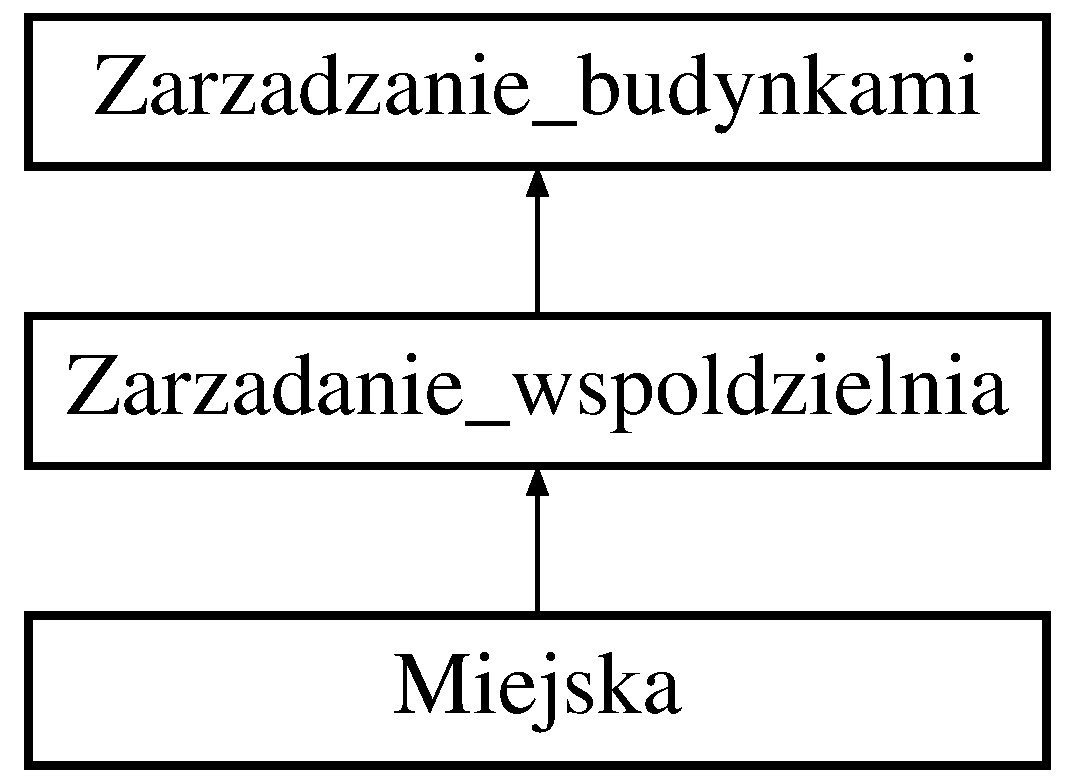
\includegraphics[height=3.000000cm]{class_miejska}
\end{center}
\end{figure}
\subsection*{Public Member Functions}
\begin{DoxyCompactItemize}
\item 
\hypertarget{class_miejska_a4bb8515d8f11cad4257d2a02b7bd1281}{}void \hyperlink{class_miejska_a4bb8515d8f11cad4257d2a02b7bd1281}{wczytaj\+\_\+z\+Pliku} ()\label{class_miejska_a4bb8515d8f11cad4257d2a02b7bd1281}

\begin{DoxyCompactList}\small\item\em Funkcja umozliwiajaca wczytanie stanu obiektu z pliku. \end{DoxyCompactList}\item 
\hypertarget{class_miejska_af1f040b536e345773ed2928b2bf1e4ab}{}void \hyperlink{class_miejska_af1f040b536e345773ed2928b2bf1e4ab}{zapisz\+\_\+do\+Pliku} ()\label{class_miejska_af1f040b536e345773ed2928b2bf1e4ab}

\begin{DoxyCompactList}\small\item\em Funkcja umozliwiajaca zapisanie stanu obiektu do pliku. \end{DoxyCompactList}\item 
\hypertarget{class_miejska_a65dd0667980bf5acba0bedfaccc4c3d0}{}void \hyperlink{class_miejska_a65dd0667980bf5acba0bedfaccc4c3d0}{dodaj\+\_\+sklep} ()\label{class_miejska_a65dd0667980bf5acba0bedfaccc4c3d0}

\begin{DoxyCompactList}\small\item\em Funkcja umozliwiajaca dodanie sklepu do spoldzielni. \end{DoxyCompactList}\item 
\hypertarget{class_miejska_a20d6ce9ea02e64a5d7f56a5cf68cd805}{}void \hyperlink{class_miejska_a20d6ce9ea02e64a5d7f56a5cf68cd805}{usun\+\_\+sklep} ()\label{class_miejska_a20d6ce9ea02e64a5d7f56a5cf68cd805}

\begin{DoxyCompactList}\small\item\em Funkcja umozliwiajaca usuniecie sklepu ze spoldzielni. \end{DoxyCompactList}\item 
\hypertarget{class_miejska_a373f0c2f745c62ffaa281a2acfa87b2e}{}void \hyperlink{class_miejska_a373f0c2f745c62ffaa281a2acfa87b2e}{wyswietl\+\_\+liste\+\_\+sklepow} ()\label{class_miejska_a373f0c2f745c62ffaa281a2acfa87b2e}

\begin{DoxyCompactList}\small\item\em Funkcja wypisujaca liste sklepow. \end{DoxyCompactList}\end{DoxyCompactItemize}
\subsection*{Additional Inherited Members}


\subsection{Detailed Description}
Klasa miejska, dziedziczaca po klasie Zarzadzanie\+\_\+wspoldzielnia. 

Klasa poszerzajaca klase bazowa o posiadanie pasazu handlowego (zbioru sklepow). 

The documentation for this class was generated from the following file\+:\begin{DoxyCompactItemize}
\item 
/home/kamil/\+Pulpit/\+Elka/\+P\+R\+O\+E/\+P\+R\+O\+E-\/2/include/Miejska.\+h\end{DoxyCompactItemize}

\hypertarget{class_obsluga__podatkow}{}\section{Obsluga\+\_\+podatkow Class Reference}
\label{class_obsluga__podatkow}\index{Obsluga\+\_\+podatkow@{Obsluga\+\_\+podatkow}}


Klasa umozliwiajaca obsluge podatkow.  




{\ttfamily \#include $<$Obsluga\+\_\+podatkow.\+h$>$}

\subsection*{Public Member Functions}
\begin{DoxyCompactItemize}
\item 
\hypertarget{class_obsluga__podatkow_a634b84304c45d982d0b164c4bf8cf00e}{}\hyperlink{class_obsluga__podatkow_a634b84304c45d982d0b164c4bf8cf00e}{Obsluga\+\_\+podatkow} ()\label{class_obsluga__podatkow_a634b84304c45d982d0b164c4bf8cf00e}

\begin{DoxyCompactList}\small\item\em Kontruktor domyslny. \end{DoxyCompactList}\item 
void \hyperlink{class_obsluga__podatkow_a1eb458cd5aa37d5da43669465e082785}{zmien\+\_\+cene\+\_\+prad} (int, int)
\begin{DoxyCompactList}\small\item\em Funkcja umozliwiajaca zmiane oplaty za prad. \end{DoxyCompactList}\item 
void \hyperlink{class_obsluga__podatkow_a990892e62f388065b1b3de92456af182}{zmien\+\_\+cene\+\_\+gaz} (int, int)
\begin{DoxyCompactList}\small\item\em Funkcja umozliwiajaca zmiane oplaty za gaz. \end{DoxyCompactList}\item 
void \hyperlink{class_obsluga__podatkow_a4ba15afdd73eb4320208426666964a33}{zmien\+\_\+cene\+\_\+woda} (int, int)
\begin{DoxyCompactList}\small\item\em Funkcja umozliwiajaca zmiane oplaty za wode. \end{DoxyCompactList}\item 
void \hyperlink{class_obsluga__podatkow_a15a42e2796b0e854cdc45fecd7fd25ec}{zmien\+\_\+cene\+\_\+czynsz} (int, int)
\begin{DoxyCompactList}\small\item\em Funkcja umozliwiajaca zmiane oplaty za czynsz. \end{DoxyCompactList}\item 
int \hyperlink{class_obsluga__podatkow_a4dffa344e102b4c31943eb4cd0d8e717}{zwroc\+\_\+cene\+\_\+prad} (int)
\begin{DoxyCompactList}\small\item\em Funkcja zwracajaca oplaty za prad. \end{DoxyCompactList}\item 
int \hyperlink{class_obsluga__podatkow_ab800b960d0092dfb382f516907a36d57}{zwroc\+\_\+cene\+\_\+gaz} (int)
\begin{DoxyCompactList}\small\item\em Funkcja zwracajaca oplaty za gaz. \end{DoxyCompactList}\item 
int \hyperlink{class_obsluga__podatkow_a873587df8807a3964724b825c2a60272}{zwroc\+\_\+cene\+\_\+woda} (int)
\begin{DoxyCompactList}\small\item\em Funkcja zwracajaca oplaty za wode. \end{DoxyCompactList}\item 
int \hyperlink{class_obsluga__podatkow_a322f0e50968dfd1bfdc2e2ee84672c26}{zwroc\+\_\+cene\+\_\+czynsz} (int)
\begin{DoxyCompactList}\small\item\em Funkcja zwracajaca oplaty za czynsz. \end{DoxyCompactList}\item 
\hypertarget{class_obsluga__podatkow_a8b4b1381191748664b9196f11429eb8c}{}void \hyperlink{class_obsluga__podatkow_a8b4b1381191748664b9196f11429eb8c}{wczytaj\+\_\+z\+Pliku} (istream \&)\label{class_obsluga__podatkow_a8b4b1381191748664b9196f11429eb8c}

\begin{DoxyCompactList}\small\item\em Funkcja umozliwiajaca wczytanie stanu obiektu z pliku. \end{DoxyCompactList}\item 
\hypertarget{class_obsluga__podatkow_a585a36ed435b2a623d0d76911ce7a5c6}{}void \hyperlink{class_obsluga__podatkow_a585a36ed435b2a623d0d76911ce7a5c6}{zapisz\+\_\+do\+Pliku} (string)\label{class_obsluga__podatkow_a585a36ed435b2a623d0d76911ce7a5c6}

\begin{DoxyCompactList}\small\item\em Funkcja umozliwiajaca zapisanie stanu obiektu do pliku. \end{DoxyCompactList}\end{DoxyCompactItemize}
\subsection*{Friends}
\begin{DoxyCompactItemize}
\item 
\hypertarget{class_obsluga__podatkow_a4fc169c719017008b6bcd0527622d787}{}ostream \& \hyperlink{class_obsluga__podatkow_a4fc169c719017008b6bcd0527622d787}{operator$<$$<$} (ostream \&, \hyperlink{class_obsluga__podatkow}{Obsluga\+\_\+podatkow} \&)\label{class_obsluga__podatkow_a4fc169c719017008b6bcd0527622d787}

\begin{DoxyCompactList}\small\item\em Operator strumieniowy. \end{DoxyCompactList}\item 
\hypertarget{class_obsluga__podatkow_a4c641271170d7967f22217bc47fc8c54}{}istream \& \hyperlink{class_obsluga__podatkow_a4c641271170d7967f22217bc47fc8c54}{operator$>$$>$} (istream \&, \hyperlink{class_obsluga__podatkow}{Obsluga\+\_\+podatkow} \&)\label{class_obsluga__podatkow_a4c641271170d7967f22217bc47fc8c54}

\begin{DoxyCompactList}\small\item\em Operator strumieniowy. \end{DoxyCompactList}\end{DoxyCompactItemize}


\subsection{Detailed Description}
Klasa umozliwiajaca obsluge podatkow. 

Zawiera informacje o podatkach, umozliwia zmiane wysokosci podatkow. 

\subsection{Member Function Documentation}
\hypertarget{class_obsluga__podatkow_a15a42e2796b0e854cdc45fecd7fd25ec}{}\index{Obsluga\+\_\+podatkow@{Obsluga\+\_\+podatkow}!zmien\+\_\+cene\+\_\+czynsz@{zmien\+\_\+cene\+\_\+czynsz}}
\index{zmien\+\_\+cene\+\_\+czynsz@{zmien\+\_\+cene\+\_\+czynsz}!Obsluga\+\_\+podatkow@{Obsluga\+\_\+podatkow}}
\subsubsection[{zmien\+\_\+cene\+\_\+czynsz(int, int)}]{\setlength{\rightskip}{0pt plus 5cm}void Obsluga\+\_\+podatkow\+::zmien\+\_\+cene\+\_\+czynsz (
\begin{DoxyParamCaption}
\item[{int}]{, }
\item[{int}]{}
\end{DoxyParamCaption}
)}\label{class_obsluga__podatkow_a15a42e2796b0e854cdc45fecd7fd25ec}


Funkcja umozliwiajaca zmiane oplaty za czynsz. 


\begin{DoxyParams}{Parameters}
{\em rodzaj} & budynku (1.\+Dom; 2.\+Szeregowiec; 3.\+Budynek; 4.\+Wiezowiec) , wysokosc oplaty. \\
\hline
\end{DoxyParams}
\hypertarget{class_obsluga__podatkow_a990892e62f388065b1b3de92456af182}{}\index{Obsluga\+\_\+podatkow@{Obsluga\+\_\+podatkow}!zmien\+\_\+cene\+\_\+gaz@{zmien\+\_\+cene\+\_\+gaz}}
\index{zmien\+\_\+cene\+\_\+gaz@{zmien\+\_\+cene\+\_\+gaz}!Obsluga\+\_\+podatkow@{Obsluga\+\_\+podatkow}}
\subsubsection[{zmien\+\_\+cene\+\_\+gaz(int, int)}]{\setlength{\rightskip}{0pt plus 5cm}void Obsluga\+\_\+podatkow\+::zmien\+\_\+cene\+\_\+gaz (
\begin{DoxyParamCaption}
\item[{int}]{, }
\item[{int}]{}
\end{DoxyParamCaption}
)}\label{class_obsluga__podatkow_a990892e62f388065b1b3de92456af182}


Funkcja umozliwiajaca zmiane oplaty za gaz. 


\begin{DoxyParams}{Parameters}
{\em rodzaj} & budynku (1.\+Dom; 2.\+Szeregowiec; 3.\+Budynek; 4.\+Wiezowiec) , wysokosc oplaty. \\
\hline
\end{DoxyParams}
\hypertarget{class_obsluga__podatkow_a1eb458cd5aa37d5da43669465e082785}{}\index{Obsluga\+\_\+podatkow@{Obsluga\+\_\+podatkow}!zmien\+\_\+cene\+\_\+prad@{zmien\+\_\+cene\+\_\+prad}}
\index{zmien\+\_\+cene\+\_\+prad@{zmien\+\_\+cene\+\_\+prad}!Obsluga\+\_\+podatkow@{Obsluga\+\_\+podatkow}}
\subsubsection[{zmien\+\_\+cene\+\_\+prad(int, int)}]{\setlength{\rightskip}{0pt plus 5cm}void Obsluga\+\_\+podatkow\+::zmien\+\_\+cene\+\_\+prad (
\begin{DoxyParamCaption}
\item[{int}]{, }
\item[{int}]{}
\end{DoxyParamCaption}
)}\label{class_obsluga__podatkow_a1eb458cd5aa37d5da43669465e082785}


Funkcja umozliwiajaca zmiane oplaty za prad. 


\begin{DoxyParams}{Parameters}
{\em rodzaj} & budynku (1.\+Dom; 2.\+Szeregowiec; 3.\+Budynek; 4.\+Wiezowiec) , wysokosc oplaty. \\
\hline
\end{DoxyParams}
\hypertarget{class_obsluga__podatkow_a4ba15afdd73eb4320208426666964a33}{}\index{Obsluga\+\_\+podatkow@{Obsluga\+\_\+podatkow}!zmien\+\_\+cene\+\_\+woda@{zmien\+\_\+cene\+\_\+woda}}
\index{zmien\+\_\+cene\+\_\+woda@{zmien\+\_\+cene\+\_\+woda}!Obsluga\+\_\+podatkow@{Obsluga\+\_\+podatkow}}
\subsubsection[{zmien\+\_\+cene\+\_\+woda(int, int)}]{\setlength{\rightskip}{0pt plus 5cm}void Obsluga\+\_\+podatkow\+::zmien\+\_\+cene\+\_\+woda (
\begin{DoxyParamCaption}
\item[{int}]{, }
\item[{int}]{}
\end{DoxyParamCaption}
)}\label{class_obsluga__podatkow_a4ba15afdd73eb4320208426666964a33}


Funkcja umozliwiajaca zmiane oplaty za wode. 


\begin{DoxyParams}{Parameters}
{\em rodzaj} & budynku (1.\+Dom; 2.\+Szeregowiec; 3.\+Budynek; 4.\+Wiezowiec) , wysokosc oplaty. \\
\hline
\end{DoxyParams}
\hypertarget{class_obsluga__podatkow_a322f0e50968dfd1bfdc2e2ee84672c26}{}\index{Obsluga\+\_\+podatkow@{Obsluga\+\_\+podatkow}!zwroc\+\_\+cene\+\_\+czynsz@{zwroc\+\_\+cene\+\_\+czynsz}}
\index{zwroc\+\_\+cene\+\_\+czynsz@{zwroc\+\_\+cene\+\_\+czynsz}!Obsluga\+\_\+podatkow@{Obsluga\+\_\+podatkow}}
\subsubsection[{zwroc\+\_\+cene\+\_\+czynsz(int)}]{\setlength{\rightskip}{0pt plus 5cm}int Obsluga\+\_\+podatkow\+::zwroc\+\_\+cene\+\_\+czynsz (
\begin{DoxyParamCaption}
\item[{int}]{}
\end{DoxyParamCaption}
)}\label{class_obsluga__podatkow_a322f0e50968dfd1bfdc2e2ee84672c26}


Funkcja zwracajaca oplaty za czynsz. 


\begin{DoxyParams}{Parameters}
{\em rodzaj} & budynku. 1.\+Dom; 2.\+Szeregowiec; 3.\+Budynek; 4.\+Wiezowiec \\
\hline
\end{DoxyParams}
\begin{DoxyReturn}{Returns}
wysokosc oplaty 
\end{DoxyReturn}
\hypertarget{class_obsluga__podatkow_ab800b960d0092dfb382f516907a36d57}{}\index{Obsluga\+\_\+podatkow@{Obsluga\+\_\+podatkow}!zwroc\+\_\+cene\+\_\+gaz@{zwroc\+\_\+cene\+\_\+gaz}}
\index{zwroc\+\_\+cene\+\_\+gaz@{zwroc\+\_\+cene\+\_\+gaz}!Obsluga\+\_\+podatkow@{Obsluga\+\_\+podatkow}}
\subsubsection[{zwroc\+\_\+cene\+\_\+gaz(int)}]{\setlength{\rightskip}{0pt plus 5cm}int Obsluga\+\_\+podatkow\+::zwroc\+\_\+cene\+\_\+gaz (
\begin{DoxyParamCaption}
\item[{int}]{}
\end{DoxyParamCaption}
)}\label{class_obsluga__podatkow_ab800b960d0092dfb382f516907a36d57}


Funkcja zwracajaca oplaty za gaz. 


\begin{DoxyParams}{Parameters}
{\em rodzaj} & budynku. 1.\+Dom; 2.\+Szeregowiec; 3.\+Budynek; 4.\+Wiezowiec \\
\hline
\end{DoxyParams}
\begin{DoxyReturn}{Returns}
wysokosc oplaty 
\end{DoxyReturn}
\hypertarget{class_obsluga__podatkow_a4dffa344e102b4c31943eb4cd0d8e717}{}\index{Obsluga\+\_\+podatkow@{Obsluga\+\_\+podatkow}!zwroc\+\_\+cene\+\_\+prad@{zwroc\+\_\+cene\+\_\+prad}}
\index{zwroc\+\_\+cene\+\_\+prad@{zwroc\+\_\+cene\+\_\+prad}!Obsluga\+\_\+podatkow@{Obsluga\+\_\+podatkow}}
\subsubsection[{zwroc\+\_\+cene\+\_\+prad(int)}]{\setlength{\rightskip}{0pt plus 5cm}int Obsluga\+\_\+podatkow\+::zwroc\+\_\+cene\+\_\+prad (
\begin{DoxyParamCaption}
\item[{int}]{}
\end{DoxyParamCaption}
)}\label{class_obsluga__podatkow_a4dffa344e102b4c31943eb4cd0d8e717}


Funkcja zwracajaca oplaty za prad. 


\begin{DoxyParams}{Parameters}
{\em rodzaj} & budynku. 1.\+Dom; 2.\+Szeregowiec; 3.\+Budynek; 4.\+Wiezowiec \\
\hline
\end{DoxyParams}
\begin{DoxyReturn}{Returns}
wysokosc oplaty 
\end{DoxyReturn}
\hypertarget{class_obsluga__podatkow_a873587df8807a3964724b825c2a60272}{}\index{Obsluga\+\_\+podatkow@{Obsluga\+\_\+podatkow}!zwroc\+\_\+cene\+\_\+woda@{zwroc\+\_\+cene\+\_\+woda}}
\index{zwroc\+\_\+cene\+\_\+woda@{zwroc\+\_\+cene\+\_\+woda}!Obsluga\+\_\+podatkow@{Obsluga\+\_\+podatkow}}
\subsubsection[{zwroc\+\_\+cene\+\_\+woda(int)}]{\setlength{\rightskip}{0pt plus 5cm}int Obsluga\+\_\+podatkow\+::zwroc\+\_\+cene\+\_\+woda (
\begin{DoxyParamCaption}
\item[{int}]{}
\end{DoxyParamCaption}
)}\label{class_obsluga__podatkow_a873587df8807a3964724b825c2a60272}


Funkcja zwracajaca oplaty za wode. 


\begin{DoxyParams}{Parameters}
{\em rodzaj} & budynku. 1.\+Dom; 2.\+Szeregowiec; 3.\+Budynek; 4.\+Wiezowiec \\
\hline
\end{DoxyParams}
\begin{DoxyReturn}{Returns}
wysokosc oplaty 
\end{DoxyReturn}


The documentation for this class was generated from the following file\+:\begin{DoxyCompactItemize}
\item 
/home/kamil/\+Pulpit/\+Elka/\+P\+R\+O\+E/\+P\+R\+O\+E-\/2/include/Obsluga\+\_\+podatkow.\+h\end{DoxyCompactItemize}

\hypertarget{class_remiza}{}\section{Remiza Class Reference}
\label{class_remiza}\index{Remiza@{Remiza}}


Klasa symulujaca wiejska remize.  




{\ttfamily \#include $<$Remiza.\+h$>$}

\subsection*{Public Member Functions}
\begin{DoxyCompactItemize}
\item 
\hypertarget{class_remiza_aa2bef7d6f557eb6bc9bc4365d7713bca}{}\hyperlink{class_remiza_aa2bef7d6f557eb6bc9bc4365d7713bca}{Remiza} ()\label{class_remiza_aa2bef7d6f557eb6bc9bc4365d7713bca}

\begin{DoxyCompactList}\small\item\em Konstruktor domyslny. \end{DoxyCompactList}\item 
void \hyperlink{class_remiza_a6c03e80da0f29066b0a441df5acc9b74}{zwieksz\+\_\+liczbe\+\_\+krzesel} (int)
\begin{DoxyCompactList}\small\item\em Zwieksza liczbe krzesel w remizie. \end{DoxyCompactList}\item 
void \hyperlink{class_remiza_a1c60448ce04370e2205263bd712b4751}{zwieksz\+\_\+liczbe\+\_\+stolikow} (int)
\begin{DoxyCompactList}\small\item\em Zwieksza liczbe stolikow w remizie. \end{DoxyCompactList}\item 
\hypertarget{class_remiza_abe72d8ccb83ad8d6cf92e16f45c6f002}{}void \hyperlink{class_remiza_abe72d8ccb83ad8d6cf92e16f45c6f002}{kup\+\_\+stol\+\_\+bilardowy} ()\label{class_remiza_abe72d8ccb83ad8d6cf92e16f45c6f002}

\begin{DoxyCompactList}\small\item\em Funkcja umozliwiajaca dodanie stolu bilarowego do remizy. \end{DoxyCompactList}\item 
\hypertarget{class_remiza_aac18782e8f1117238858db4d5f21cd50}{}void \hyperlink{class_remiza_aac18782e8f1117238858db4d5f21cd50}{kup\+\_\+stol\+\_\+pingpongowy} ()\label{class_remiza_aac18782e8f1117238858db4d5f21cd50}

\begin{DoxyCompactList}\small\item\em Funkcja umozliwiajaca dodanie stolu pingpongowego do remizy. \end{DoxyCompactList}\item 
\hypertarget{class_remiza_a783c6296060a050b61935787794d027c}{}void \hyperlink{class_remiza_a783c6296060a050b61935787794d027c}{wczytaj\+\_\+z\+Pliku} (istream \&)\label{class_remiza_a783c6296060a050b61935787794d027c}

\begin{DoxyCompactList}\small\item\em Funkcja umozliwiajaca wczytanie stanu obiektu z pliku. \end{DoxyCompactList}\item 
\hypertarget{class_remiza_a4c2563c5bde280b2232a555f45f79b3b}{}void \hyperlink{class_remiza_a4c2563c5bde280b2232a555f45f79b3b}{zapisz\+\_\+do\+Pliku} (string)\label{class_remiza_a4c2563c5bde280b2232a555f45f79b3b}

\begin{DoxyCompactList}\small\item\em Funkcja umozliwiajaca zapisanie stanu obiektu do pliku. \end{DoxyCompactList}\item 
int \hyperlink{class_remiza_ac7525b855d2ca06358f4f85eec6e712f}{ile\+\_\+krzesel} ()
\begin{DoxyCompactList}\small\item\em Funkcja zwracajaca ilosc krzesel. \end{DoxyCompactList}\item 
int \hyperlink{class_remiza_a58e9ad55b9a48892ab9d69e728d53e41}{ile\+\_\+stolikow} ()
\begin{DoxyCompactList}\small\item\em Funkcja zwracajaca ilosc stolikow. \end{DoxyCompactList}\item 
bool \hyperlink{class_remiza_a20b0ebdb1a93fd34a1b8d7c645d364b0}{czy\+\_\+jest\+\_\+bilard} ()
\begin{DoxyCompactList}\small\item\em Funkcja zwracajaca informacje czy jest bilard w remizie. \end{DoxyCompactList}\item 
bool \hyperlink{class_remiza_a19d23b5a0b58b717ceeaeb094d6214a2}{czy\+\_\+jest\+\_\+pingpong} ()
\begin{DoxyCompactList}\small\item\em Funkcja zwracajaca informacje czy jest pingpong w remizie. \end{DoxyCompactList}\item 
\hypertarget{class_remiza_acb8a536322f8998455c74c3c2abf4c38}{}void \hyperlink{class_remiza_acb8a536322f8998455c74c3c2abf4c38}{info\+\_\+remiza} ()\label{class_remiza_acb8a536322f8998455c74c3c2abf4c38}

\begin{DoxyCompactList}\small\item\em Funkcja wyswietlajaca informacje o remizie. \end{DoxyCompactList}\end{DoxyCompactItemize}
\subsection*{Friends}
\begin{DoxyCompactItemize}
\item 
\hypertarget{class_remiza_a05fabcfc7697eba73829af6e16d6c8cf}{}ostream \& \hyperlink{class_remiza_a05fabcfc7697eba73829af6e16d6c8cf}{operator$<$$<$} (ostream \&, \hyperlink{class_remiza}{Remiza} \&)\label{class_remiza_a05fabcfc7697eba73829af6e16d6c8cf}

\begin{DoxyCompactList}\small\item\em Operator strumieniowy. \end{DoxyCompactList}\item 
\hypertarget{class_remiza_a99a5a20cd89c0b02ce969971ee348a83}{}istream \& \hyperlink{class_remiza_a99a5a20cd89c0b02ce969971ee348a83}{operator$>$$>$} (istream \&, \hyperlink{class_remiza}{Remiza} \&)\label{class_remiza_a99a5a20cd89c0b02ce969971ee348a83}

\begin{DoxyCompactList}\small\item\em Operator strumieniowy. \end{DoxyCompactList}\end{DoxyCompactItemize}


\subsection{Detailed Description}
Klasa symulujaca wiejska remize. 

\subsection{Member Function Documentation}
\hypertarget{class_remiza_a20b0ebdb1a93fd34a1b8d7c645d364b0}{}\index{Remiza@{Remiza}!czy\+\_\+jest\+\_\+bilard@{czy\+\_\+jest\+\_\+bilard}}
\index{czy\+\_\+jest\+\_\+bilard@{czy\+\_\+jest\+\_\+bilard}!Remiza@{Remiza}}
\subsubsection[{czy\+\_\+jest\+\_\+bilard()}]{\setlength{\rightskip}{0pt plus 5cm}bool Remiza\+::czy\+\_\+jest\+\_\+bilard (
\begin{DoxyParamCaption}
{}
\end{DoxyParamCaption}
)}\label{class_remiza_a20b0ebdb1a93fd34a1b8d7c645d364b0}


Funkcja zwracajaca informacje czy jest bilard w remizie. 

Tak -\/ True, Nie -\/ False \hypertarget{class_remiza_a19d23b5a0b58b717ceeaeb094d6214a2}{}\index{Remiza@{Remiza}!czy\+\_\+jest\+\_\+pingpong@{czy\+\_\+jest\+\_\+pingpong}}
\index{czy\+\_\+jest\+\_\+pingpong@{czy\+\_\+jest\+\_\+pingpong}!Remiza@{Remiza}}
\subsubsection[{czy\+\_\+jest\+\_\+pingpong()}]{\setlength{\rightskip}{0pt plus 5cm}bool Remiza\+::czy\+\_\+jest\+\_\+pingpong (
\begin{DoxyParamCaption}
{}
\end{DoxyParamCaption}
)}\label{class_remiza_a19d23b5a0b58b717ceeaeb094d6214a2}


Funkcja zwracajaca informacje czy jest pingpong w remizie. 

Tak -\/ True, Nie -\/ False \hypertarget{class_remiza_ac7525b855d2ca06358f4f85eec6e712f}{}\index{Remiza@{Remiza}!ile\+\_\+krzesel@{ile\+\_\+krzesel}}
\index{ile\+\_\+krzesel@{ile\+\_\+krzesel}!Remiza@{Remiza}}
\subsubsection[{ile\+\_\+krzesel()}]{\setlength{\rightskip}{0pt plus 5cm}int Remiza\+::ile\+\_\+krzesel (
\begin{DoxyParamCaption}
{}
\end{DoxyParamCaption}
)}\label{class_remiza_ac7525b855d2ca06358f4f85eec6e712f}


Funkcja zwracajaca ilosc krzesel. 

\begin{DoxyReturn}{Returns}
ilosc krzesel 
\end{DoxyReturn}
\hypertarget{class_remiza_a58e9ad55b9a48892ab9d69e728d53e41}{}\index{Remiza@{Remiza}!ile\+\_\+stolikow@{ile\+\_\+stolikow}}
\index{ile\+\_\+stolikow@{ile\+\_\+stolikow}!Remiza@{Remiza}}
\subsubsection[{ile\+\_\+stolikow()}]{\setlength{\rightskip}{0pt plus 5cm}int Remiza\+::ile\+\_\+stolikow (
\begin{DoxyParamCaption}
{}
\end{DoxyParamCaption}
)}\label{class_remiza_a58e9ad55b9a48892ab9d69e728d53e41}


Funkcja zwracajaca ilosc stolikow. 

\begin{DoxyReturn}{Returns}
ilosc stolikow 
\end{DoxyReturn}
\hypertarget{class_remiza_a6c03e80da0f29066b0a441df5acc9b74}{}\index{Remiza@{Remiza}!zwieksz\+\_\+liczbe\+\_\+krzesel@{zwieksz\+\_\+liczbe\+\_\+krzesel}}
\index{zwieksz\+\_\+liczbe\+\_\+krzesel@{zwieksz\+\_\+liczbe\+\_\+krzesel}!Remiza@{Remiza}}
\subsubsection[{zwieksz\+\_\+liczbe\+\_\+krzesel(int)}]{\setlength{\rightskip}{0pt plus 5cm}void Remiza\+::zwieksz\+\_\+liczbe\+\_\+krzesel (
\begin{DoxyParamCaption}
\item[{int}]{}
\end{DoxyParamCaption}
)}\label{class_remiza_a6c03e80da0f29066b0a441df5acc9b74}


Zwieksza liczbe krzesel w remizie. 


\begin{DoxyParams}{Parameters}
{\em Informacja} & o ile zwiekszamy ilosc krzesel. \\
\hline
\end{DoxyParams}
\hypertarget{class_remiza_a1c60448ce04370e2205263bd712b4751}{}\index{Remiza@{Remiza}!zwieksz\+\_\+liczbe\+\_\+stolikow@{zwieksz\+\_\+liczbe\+\_\+stolikow}}
\index{zwieksz\+\_\+liczbe\+\_\+stolikow@{zwieksz\+\_\+liczbe\+\_\+stolikow}!Remiza@{Remiza}}
\subsubsection[{zwieksz\+\_\+liczbe\+\_\+stolikow(int)}]{\setlength{\rightskip}{0pt plus 5cm}void Remiza\+::zwieksz\+\_\+liczbe\+\_\+stolikow (
\begin{DoxyParamCaption}
\item[{int}]{}
\end{DoxyParamCaption}
)}\label{class_remiza_a1c60448ce04370e2205263bd712b4751}


Zwieksza liczbe stolikow w remizie. 


\begin{DoxyParams}{Parameters}
{\em Informacja} & o ile zwiekszamy ilosc stolikow. \\
\hline
\end{DoxyParams}


The documentation for this class was generated from the following file\+:\begin{DoxyCompactItemize}
\item 
/home/kamil/\+Pulpit/\+Elka/\+P\+R\+O\+E/\+P\+R\+O\+E-\/2/include/Remiza.\+h\end{DoxyCompactItemize}

\hypertarget{class_sklep}{}\section{Sklep Class Reference}
\label{class_sklep}\index{Sklep@{Sklep}}


Klasa \hyperlink{class_sklep}{Sklep}, poszerzajaca mozliwosci Budynku o informacje o sklepie. Domyslnie jej rodzaj to 1.  




{\ttfamily \#include $<$Sklep.\+h$>$}

Inheritance diagram for Sklep\+:\begin{figure}[H]
\begin{center}
\leavevmode
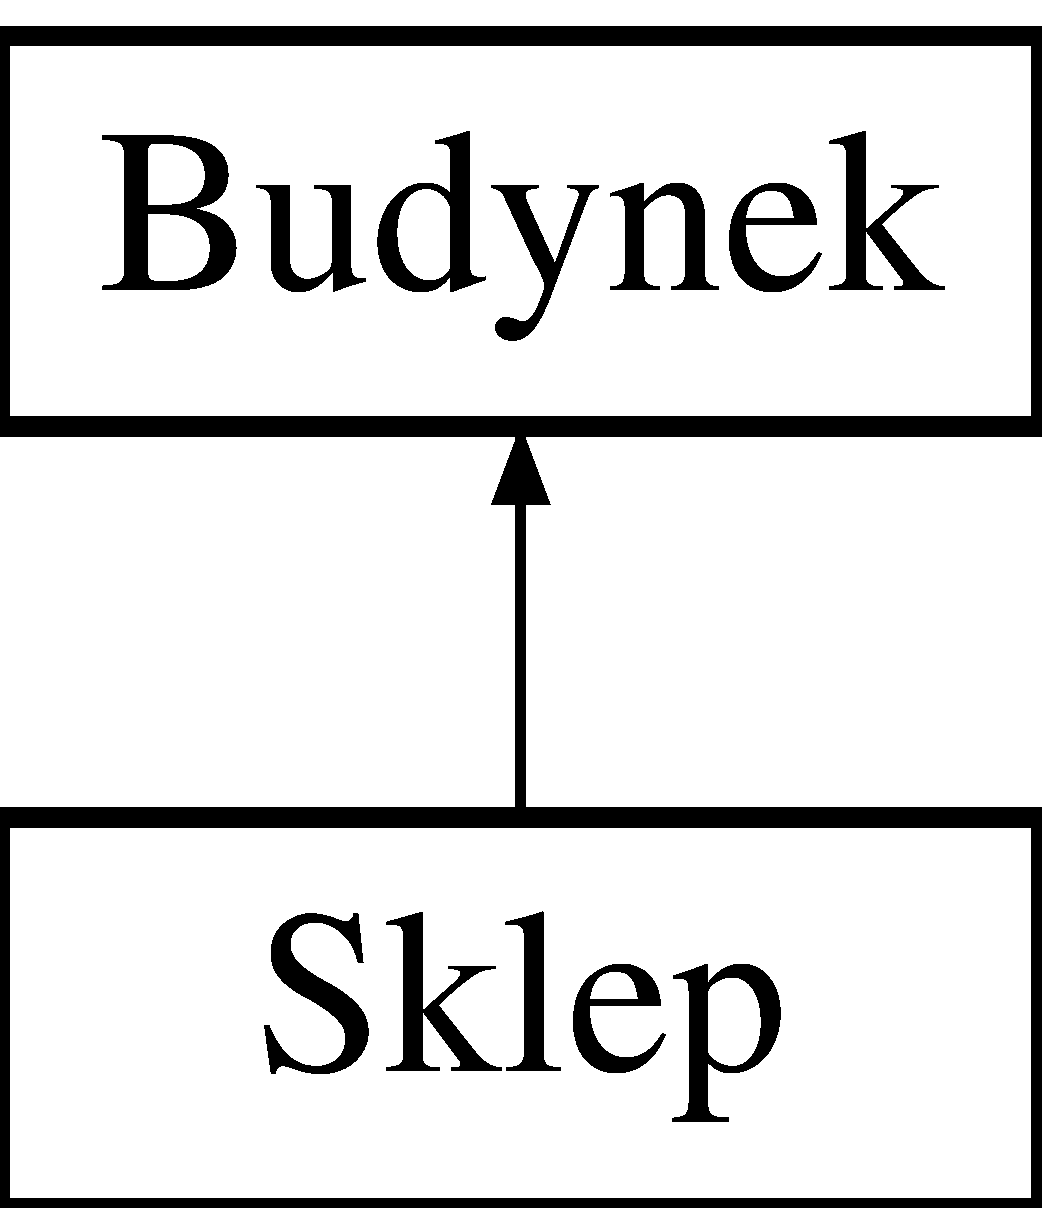
\includegraphics[height=2.000000cm]{class_sklep}
\end{center}
\end{figure}
\subsection*{Public Member Functions}
\begin{DoxyCompactItemize}
\item 
\hypertarget{class_sklep_af38b90089cdb38d64032bb188a8cf1d5}{}\hyperlink{class_sklep_af38b90089cdb38d64032bb188a8cf1d5}{Sklep} (char s=0, string rs=\char`\"{}Zwykly\char`\"{})\label{class_sklep_af38b90089cdb38d64032bb188a8cf1d5}

\begin{DoxyCompactList}\small\item\em Konstruktor. \end{DoxyCompactList}\item 
\hypertarget{class_sklep_a37ceeb8a28621956abd723c138d8f959}{}void \hyperlink{class_sklep_a37ceeb8a28621956abd723c138d8f959}{wczytaj\+\_\+z\+Pliku} (istream \&)\label{class_sklep_a37ceeb8a28621956abd723c138d8f959}

\begin{DoxyCompactList}\small\item\em Funkcja umozliwiajaca wczytanie stanu obiektu z pliku. \end{DoxyCompactList}\item 
\hypertarget{class_sklep_a5cec36bf246569297492661ef183baa0}{}void \hyperlink{class_sklep_a5cec36bf246569297492661ef183baa0}{zapisz\+\_\+do\+Pliku} (string)\label{class_sklep_a5cec36bf246569297492661ef183baa0}

\begin{DoxyCompactList}\small\item\em Funkcja umozliwiajaca zapisanie stanu obiektu do pliku. \end{DoxyCompactList}\item 
string \hyperlink{class_sklep_a70447391a0f4d141ee24af47ac1939f7}{zwroc\+\_\+rodzaj\+\_\+sklepu} ()
\begin{DoxyCompactList}\small\item\em Funkcja zwracajaca rodzaj sklepu. \end{DoxyCompactList}\end{DoxyCompactItemize}
\subsection*{Additional Inherited Members}


\subsection{Detailed Description}
Klasa \hyperlink{class_sklep}{Sklep}, poszerzajaca mozliwosci Budynku o informacje o sklepie. Domyslnie jej rodzaj to 1. 

\subsection{Member Function Documentation}
\hypertarget{class_sklep_a70447391a0f4d141ee24af47ac1939f7}{}\index{Sklep@{Sklep}!zwroc\+\_\+rodzaj\+\_\+sklepu@{zwroc\+\_\+rodzaj\+\_\+sklepu}}
\index{zwroc\+\_\+rodzaj\+\_\+sklepu@{zwroc\+\_\+rodzaj\+\_\+sklepu}!Sklep@{Sklep}}
\subsubsection[{zwroc\+\_\+rodzaj\+\_\+sklepu()}]{\setlength{\rightskip}{0pt plus 5cm}string Sklep\+::zwroc\+\_\+rodzaj\+\_\+sklepu (
\begin{DoxyParamCaption}
{}
\end{DoxyParamCaption}
)}\label{class_sklep_a70447391a0f4d141ee24af47ac1939f7}


Funkcja zwracajaca rodzaj sklepu. 

\begin{DoxyReturn}{Returns}
rodzaj sklepu. 
\end{DoxyReturn}


The documentation for this class was generated from the following file\+:\begin{DoxyCompactItemize}
\item 
/home/kamil/\+Pulpit/\+Elka/\+P\+R\+O\+E/\+P\+R\+O\+E-\/2/include/Sklep.\+h\end{DoxyCompactItemize}

\hypertarget{class_wiejska}{}\section{Wiejska Class Reference}
\label{class_wiejska}\index{Wiejska@{Wiejska}}


Klasa wiejska poszerze mozliwosci klasy bazowej o posiadanie \char`\"{}remizy\char`\"{}.  




{\ttfamily \#include $<$Wiejska.\+h$>$}

Inheritance diagram for Wiejska\+:\begin{figure}[H]
\begin{center}
\leavevmode
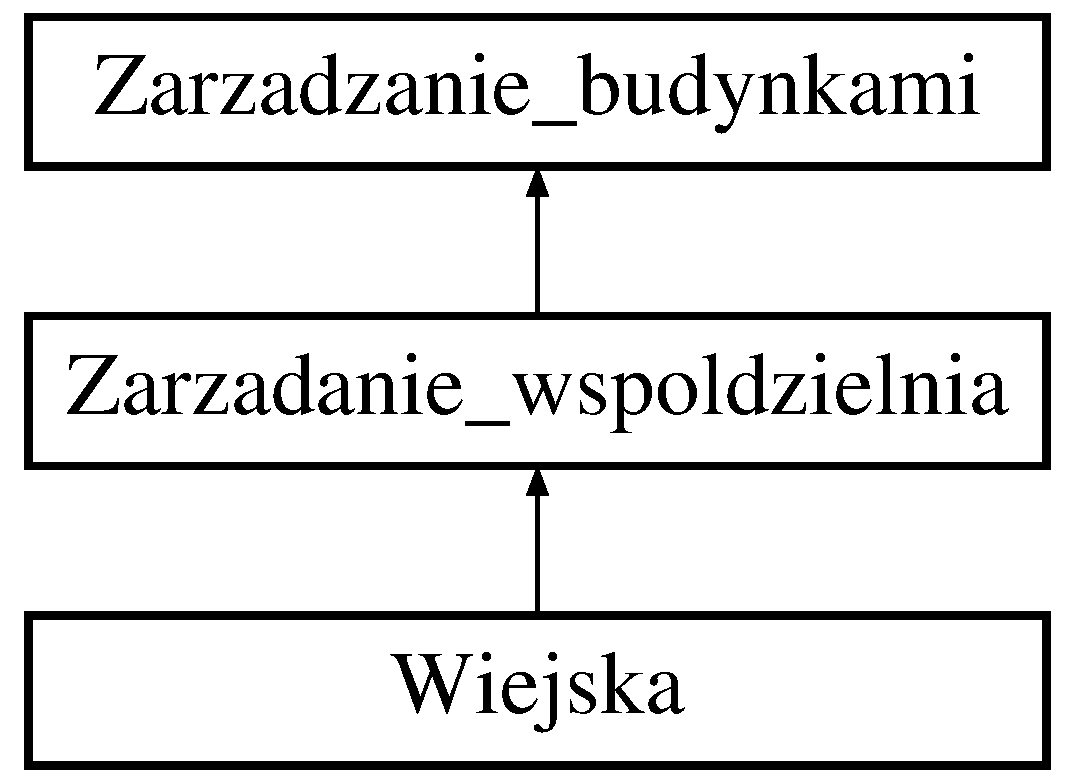
\includegraphics[height=3.000000cm]{class_wiejska}
\end{center}
\end{figure}
\subsection*{Public Member Functions}
\begin{DoxyCompactItemize}
\item 
\hypertarget{class_wiejska_a0ca71e49d6503eba63a04e12a3f3539f}{}void \hyperlink{class_wiejska_a0ca71e49d6503eba63a04e12a3f3539f}{wczytaj\+\_\+z\+Pliku} ()\label{class_wiejska_a0ca71e49d6503eba63a04e12a3f3539f}

\begin{DoxyCompactList}\small\item\em Funkcja czysto wirtualna, umozliwiajaca wczytanie z pliku. \end{DoxyCompactList}\item 
\hypertarget{class_wiejska_a625c01c80cc223184a2e3c50b7749c96}{}void \hyperlink{class_wiejska_a625c01c80cc223184a2e3c50b7749c96}{zapisz\+\_\+do\+Pliku} ()\label{class_wiejska_a625c01c80cc223184a2e3c50b7749c96}

\begin{DoxyCompactList}\small\item\em Funkcja czysto wirtualna, umozliwiajaca zapisanie do pliku. \end{DoxyCompactList}\item 
\hypertarget{class_wiejska_adedd94a38deb6f196a0966d477d404f2}{}void \hyperlink{class_wiejska_adedd94a38deb6f196a0966d477d404f2}{kup\+\_\+krzesla} ()\label{class_wiejska_adedd94a38deb6f196a0966d477d404f2}

\begin{DoxyCompactList}\small\item\em Funkcja umozliwiajaca dodanie krzesel. \end{DoxyCompactList}\item 
\hypertarget{class_wiejska_adc172ccf73df677e0d343faab76a9952}{}void \hyperlink{class_wiejska_adc172ccf73df677e0d343faab76a9952}{kup\+\_\+stoliki} ()\label{class_wiejska_adc172ccf73df677e0d343faab76a9952}

\begin{DoxyCompactList}\small\item\em Funkcja umozliwiajaca dodanie stolikow. \end{DoxyCompactList}\item 
\hypertarget{class_wiejska_a9b28e7cff9b4706522205fcda30371cc}{}void \hyperlink{class_wiejska_a9b28e7cff9b4706522205fcda30371cc}{kup\+\_\+stol\+\_\+bilardowy} ()\label{class_wiejska_a9b28e7cff9b4706522205fcda30371cc}

\begin{DoxyCompactList}\small\item\em Funkcja umozliwiajaca dodanie stolu bilardowego. \end{DoxyCompactList}\item 
\hypertarget{class_wiejska_a08bdb7517c1f7df61993db56adbc1c74}{}void \hyperlink{class_wiejska_a08bdb7517c1f7df61993db56adbc1c74}{kup\+\_\+stol\+\_\+pingpongowy} ()\label{class_wiejska_a08bdb7517c1f7df61993db56adbc1c74}

\begin{DoxyCompactList}\small\item\em Funkcja umozliwiajaca dodanie stolu pingpongowego. \end{DoxyCompactList}\item 
\hypertarget{class_wiejska_a807a65b9b6b956d7f4a15cb463ad2a4c}{}void \hyperlink{class_wiejska_a807a65b9b6b956d7f4a15cb463ad2a4c}{info\+\_\+remiza} ()\label{class_wiejska_a807a65b9b6b956d7f4a15cb463ad2a4c}

\begin{DoxyCompactList}\small\item\em Funkcja wyswietla informacje o remizie. \end{DoxyCompactList}\item 
\hypertarget{class_wiejska_a2fb45e3f98a63f1aa0252e2daa3e3c1a}{}void \hyperlink{class_wiejska_a2fb45e3f98a63f1aa0252e2daa3e3c1a}{info\+\_\+wspoldzielnia} ()\label{class_wiejska_a2fb45e3f98a63f1aa0252e2daa3e3c1a}

\begin{DoxyCompactList}\small\item\em Funkcja wyswietlajaca informacje i spoldzielni. \end{DoxyCompactList}\end{DoxyCompactItemize}
\subsection*{Additional Inherited Members}


\subsection{Detailed Description}
Klasa wiejska poszerze mozliwosci klasy bazowej o posiadanie \char`\"{}remizy\char`\"{}. 

The documentation for this class was generated from the following file\+:\begin{DoxyCompactItemize}
\item 
/home/kamil/\+Pulpit/\+Elka/\+P\+R\+O\+E/\+P\+R\+O\+E-\/2/include/Wiejska.\+h\end{DoxyCompactItemize}

\hypertarget{class_zarzadanie__wspoldzielnia}{}\section{Zarzadanie\+\_\+wspoldzielnia Class Reference}
\label{class_zarzadanie__wspoldzielnia}\index{Zarzadanie\+\_\+wspoldzielnia@{Zarzadanie\+\_\+wspoldzielnia}}


Klasa bazowa, projektu. Symuluje dzialanie Spoldzielni mieszkaniowej.  




{\ttfamily \#include $<$Zarzadzanie\+\_\+wspoldzielnia.\+h$>$}

Inheritance diagram for Zarzadanie\+\_\+wspoldzielnia\+:\begin{figure}[H]
\begin{center}
\leavevmode
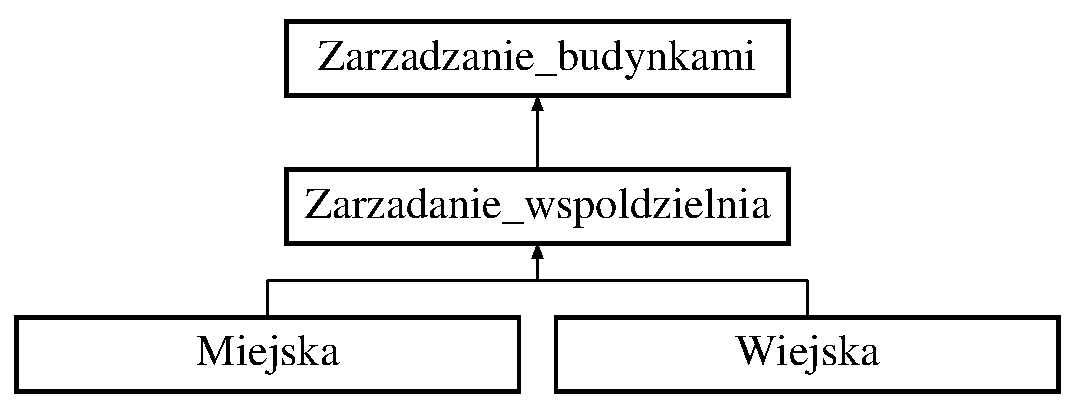
\includegraphics[height=3.000000cm]{class_zarzadanie__wspoldzielnia}
\end{center}
\end{figure}
\subsection*{Public Member Functions}
\begin{DoxyCompactItemize}
\item 
\hypertarget{class_zarzadanie__wspoldzielnia_a76e6f4fae35734588b3a66bf5b9a8b8a}{}\hyperlink{class_zarzadanie__wspoldzielnia_a76e6f4fae35734588b3a66bf5b9a8b8a}{Zarzadanie\+\_\+wspoldzielnia} ()\label{class_zarzadanie__wspoldzielnia_a76e6f4fae35734588b3a66bf5b9a8b8a}

\begin{DoxyCompactList}\small\item\em Kontruktor domyslny. \end{DoxyCompactList}\item 
\hypertarget{class_zarzadanie__wspoldzielnia_ac004989293c215e3cf877f109b5e96a0}{}void \hyperlink{class_zarzadanie__wspoldzielnia_ac004989293c215e3cf877f109b5e96a0}{wczytaj\+\_\+z\+Pliku} ()\label{class_zarzadanie__wspoldzielnia_ac004989293c215e3cf877f109b5e96a0}

\begin{DoxyCompactList}\small\item\em Funkcja umozliwiajaca wczytanie obiektu z pliku. \end{DoxyCompactList}\item 
\hypertarget{class_zarzadanie__wspoldzielnia_a54e43549dbff31055cbc81050908a895}{}void \hyperlink{class_zarzadanie__wspoldzielnia_a54e43549dbff31055cbc81050908a895}{zapisz\+\_\+do\+Pliku} ()\label{class_zarzadanie__wspoldzielnia_a54e43549dbff31055cbc81050908a895}

\begin{DoxyCompactList}\small\item\em Funkcja umozliwiajaca zapisanie obiektu do pliku. \end{DoxyCompactList}\item 
int \hyperlink{class_zarzadanie__wspoldzielnia_a7ed866ff4292827140084bd79af5f9d4}{zwroc\+\_\+stan\+\_\+konta} ()
\begin{DoxyCompactList}\small\item\em Funkcja zwracajaca stan konta spoldzielni. \end{DoxyCompactList}\item 
string \hyperlink{class_zarzadanie__wspoldzielnia_a62b6b6ffa97c782a1dd80e27e77643ea}{zwroc\+\_\+nazwe} ()
\begin{DoxyCompactList}\small\item\em Funkcja zwracajaca nazwe spoldzielni. \end{DoxyCompactList}\item 
void \hyperlink{class_zarzadanie__wspoldzielnia_a82d8de3fca3742f0e6a64ce2826a3b0e}{ustaw\+\_\+nazwe} (string)
\begin{DoxyCompactList}\small\item\em Funkcja umozliwiajaca zmiane nazwy spoldzielni. \end{DoxyCompactList}\item 
void \hyperlink{class_zarzadanie__wspoldzielnia_ae6a070fc20c47a8f2326633c5febae26}{ustaw\+\_\+stan\+\_\+konta} (int)
\begin{DoxyCompactList}\small\item\em Funkcja umozliwiajaca zmiane stanu konta spoldzielni. \end{DoxyCompactList}\item 
\hypertarget{class_zarzadanie__wspoldzielnia_a23ef8e239cc5d8563f98bc902d279c0d}{}void \hyperlink{class_zarzadanie__wspoldzielnia_a23ef8e239cc5d8563f98bc902d279c0d}{info\+\_\+wspoldzielnia} ()\label{class_zarzadanie__wspoldzielnia_a23ef8e239cc5d8563f98bc902d279c0d}

\begin{DoxyCompactList}\small\item\em Funkcja wyswietlajaca informacje o spoldzielni. \end{DoxyCompactList}\item 
\hypertarget{class_zarzadanie__wspoldzielnia_a8d5375db39f4591fd467eb370ff15338}{}void \hyperlink{class_zarzadanie__wspoldzielnia_a8d5375db39f4591fd467eb370ff15338}{wyswietl\+\_\+info\+\_\+podatki} ()\label{class_zarzadanie__wspoldzielnia_a8d5375db39f4591fd467eb370ff15338}

\begin{DoxyCompactList}\small\item\em Funkcja wyswietlajaca informacje o podatkach. \end{DoxyCompactList}\item 
\hypertarget{class_zarzadanie__wspoldzielnia_a8c74803cc1d5819e54e46c13e624d3bc}{}void \hyperlink{class_zarzadanie__wspoldzielnia_a8c74803cc1d5819e54e46c13e624d3bc}{zebranie\+\_\+podatku} ()\label{class_zarzadanie__wspoldzielnia_a8c74803cc1d5819e54e46c13e624d3bc}

\begin{DoxyCompactList}\small\item\em Funkcja umozliwiajaca wyegzekwowanie podatkow. \end{DoxyCompactList}\item 
\hypertarget{class_zarzadanie__wspoldzielnia_a79a6bd0f14276478baa8fc6811719515}{}void \hyperlink{class_zarzadanie__wspoldzielnia_a79a6bd0f14276478baa8fc6811719515}{zmien\+\_\+cene\+\_\+podatkow} ()\label{class_zarzadanie__wspoldzielnia_a79a6bd0f14276478baa8fc6811719515}

\begin{DoxyCompactList}\small\item\em Funkcja umozliwiajaca zmiane wysokosci podatkow. \end{DoxyCompactList}\item 
\hypertarget{class_zarzadanie__wspoldzielnia_a07fcd69d311fac7e1cc9dc1c34bfe65e}{}void \hyperlink{class_zarzadanie__wspoldzielnia_a07fcd69d311fac7e1cc9dc1c34bfe65e}{wyswietl\+\_\+info\+\_\+remont} ()\label{class_zarzadanie__wspoldzielnia_a07fcd69d311fac7e1cc9dc1c34bfe65e}

\begin{DoxyCompactList}\small\item\em Funkcja zwracajaca informacje o firmie remontowej spoldzielni. \end{DoxyCompactList}\item 
\hypertarget{class_zarzadanie__wspoldzielnia_ac85986ebf98ca6a13f8d163b4b100151}{}void \hyperlink{class_zarzadanie__wspoldzielnia_ac85986ebf98ca6a13f8d163b4b100151}{zmien\+\_\+nazwe\+\_\+firmy\+\_\+remontowej} ()\label{class_zarzadanie__wspoldzielnia_ac85986ebf98ca6a13f8d163b4b100151}

\begin{DoxyCompactList}\small\item\em Funkcja umozliwiajaca zmiane nazwy firmy spoldzielni. \end{DoxyCompactList}\item 
\hypertarget{class_zarzadanie__wspoldzielnia_a00b4f3b54fcb0959c7a77bbec969efea}{}void \hyperlink{class_zarzadanie__wspoldzielnia_a00b4f3b54fcb0959c7a77bbec969efea}{zmien\+\_\+ceny\+\_\+firmy\+\_\+remontowej} ()\label{class_zarzadanie__wspoldzielnia_a00b4f3b54fcb0959c7a77bbec969efea}

\begin{DoxyCompactList}\small\item\em Funkcja umozliwiajaca zmiane ceny uslug firmy remontowej. \end{DoxyCompactList}\item 
\hypertarget{class_zarzadanie__wspoldzielnia_a0280cc672c127673217e8a31de57b210}{}void \hyperlink{class_zarzadanie__wspoldzielnia_a0280cc672c127673217e8a31de57b210}{przeprowadz\+\_\+remont} ()\label{class_zarzadanie__wspoldzielnia_a0280cc672c127673217e8a31de57b210}

\begin{DoxyCompactList}\small\item\em Funkcja umozliwiajaca przeprowadzanie remontu. \end{DoxyCompactList}\item 
\hypertarget{class_zarzadanie__wspoldzielnia_a00418cfb3dde37869cc68b3daf580dff}{}\hyperlink{class_zarzadanie__wspoldzielnia}{Zarzadanie\+\_\+wspoldzielnia} \hyperlink{class_zarzadanie__wspoldzielnia_a00418cfb3dde37869cc68b3daf580dff}{operator+} (const \hyperlink{class_zarzadanie__wspoldzielnia}{Zarzadanie\+\_\+wspoldzielnia} \&)\label{class_zarzadanie__wspoldzielnia_a00418cfb3dde37869cc68b3daf580dff}

\begin{DoxyCompactList}\small\item\em Operator umozliwiajacy stworzenie nowej spoldzielni, ktora ma stan konta bedacy suma. \end{DoxyCompactList}\item 
\hypertarget{class_zarzadanie__wspoldzielnia_ad457fe5a321df131677eae6a55f439d9}{}bool \hyperlink{class_zarzadanie__wspoldzielnia_ad457fe5a321df131677eae6a55f439d9}{operator$>$} (\hyperlink{class_zarzadanie__wspoldzielnia}{Zarzadanie\+\_\+wspoldzielnia} \&)\label{class_zarzadanie__wspoldzielnia_ad457fe5a321df131677eae6a55f439d9}

\begin{DoxyCompactList}\small\item\em Operator umozliwiajacy stwierdzenie ktora spoldzielnia jest bogatsza. \end{DoxyCompactList}\item 
\hypertarget{class_zarzadanie__wspoldzielnia_a886385060b4570577f46ea42e6c6287f}{}bool \hyperlink{class_zarzadanie__wspoldzielnia_a886385060b4570577f46ea42e6c6287f}{operator$<$} (\hyperlink{class_zarzadanie__wspoldzielnia}{Zarzadanie\+\_\+wspoldzielnia} \&)\label{class_zarzadanie__wspoldzielnia_a886385060b4570577f46ea42e6c6287f}

\begin{DoxyCompactList}\small\item\em Operator umozliwiajacy stwierdzenie ktora spoldzielnia jest biedniejsza. \end{DoxyCompactList}\item 
\hypertarget{class_zarzadanie__wspoldzielnia_a5bed74d5c89f68cb887db0adfdf2c7f3}{}bool \hyperlink{class_zarzadanie__wspoldzielnia_a5bed74d5c89f68cb887db0adfdf2c7f3}{operator==} (\hyperlink{class_zarzadanie__wspoldzielnia}{Zarzadanie\+\_\+wspoldzielnia} \&)\label{class_zarzadanie__wspoldzielnia_a5bed74d5c89f68cb887db0adfdf2c7f3}

\begin{DoxyCompactList}\small\item\em Operator odpowiadajacy na pytanie czy spoldzielnie sa tak samo bogate. \end{DoxyCompactList}\item 
\hypertarget{class_zarzadanie__wspoldzielnia_a892af36fbe7745711903ad144275a13c}{}void \hyperlink{class_zarzadanie__wspoldzielnia_a892af36fbe7745711903ad144275a13c}{operator\mbox{[}$\,$\mbox{]}} (const string \&)\label{class_zarzadanie__wspoldzielnia_a892af36fbe7745711903ad144275a13c}

\begin{DoxyCompactList}\small\item\em Operator umozliwiajacy zmiane nazwy spoldzielni. \end{DoxyCompactList}\item 
\hypertarget{class_zarzadanie__wspoldzielnia_ad9646551b947b99460ca544bc7f5b2b9}{}void \hyperlink{class_zarzadanie__wspoldzielnia_ad9646551b947b99460ca544bc7f5b2b9}{operator\mbox{[}$\,$\mbox{]}} (const char\mbox{[}$\,$\mbox{]})\label{class_zarzadanie__wspoldzielnia_ad9646551b947b99460ca544bc7f5b2b9}

\begin{DoxyCompactList}\small\item\em Operator umozliwiajacy zmiane nazwy spoldzielni. \end{DoxyCompactList}\item 
\hypertarget{class_zarzadanie__wspoldzielnia_a248d69f67a8c142f3cd5f3afb8fc4ac4}{}void \hyperlink{class_zarzadanie__wspoldzielnia_a248d69f67a8c142f3cd5f3afb8fc4ac4}{operator\mbox{[}$\,$\mbox{]}} (const int)\label{class_zarzadanie__wspoldzielnia_a248d69f67a8c142f3cd5f3afb8fc4ac4}

\begin{DoxyCompactList}\small\item\em Operator umozliwiajacy zmiane wysokosci stanu konta spoldzielni. \end{DoxyCompactList}\item 
\hypertarget{class_zarzadanie__wspoldzielnia_a076ea47fd2fe403cde12c15b8341b703}{}\hyperlink{class_zarzadanie__wspoldzielnia_a076ea47fd2fe403cde12c15b8341b703}{operator int} () const \label{class_zarzadanie__wspoldzielnia_a076ea47fd2fe403cde12c15b8341b703}

\begin{DoxyCompactList}\small\item\em Operator zwracajacy stan konta spoldzielni. \end{DoxyCompactList}\item 
\hypertarget{class_zarzadanie__wspoldzielnia_a6ba5f8752ec31e14ae97a84db5abc103}{}void \hyperlink{class_zarzadanie__wspoldzielnia_a6ba5f8752ec31e14ae97a84db5abc103}{operator!} ()\label{class_zarzadanie__wspoldzielnia_a6ba5f8752ec31e14ae97a84db5abc103}

\begin{DoxyCompactList}\small\item\em Operator zerujacy obiekt. \end{DoxyCompactList}\end{DoxyCompactItemize}
\subsection*{Static Public Member Functions}
\begin{DoxyCompactItemize}
\item 
\hypertarget{class_zarzadanie__wspoldzielnia_adbe9f19e8c8df7718ab41f1e50efa646}{}static int \hyperlink{class_zarzadanie__wspoldzielnia_adbe9f19e8c8df7718ab41f1e50efa646}{zwroc\+\_\+ilosc\+\_\+obiektow} ()\label{class_zarzadanie__wspoldzielnia_adbe9f19e8c8df7718ab41f1e50efa646}

\begin{DoxyCompactList}\small\item\em Funkcja zwracajaca ilosc stworzonych obiektow tej klasy. \end{DoxyCompactList}\end{DoxyCompactItemize}
\subsection*{Protected Attributes}
\begin{DoxyCompactItemize}
\item 
\hyperlink{class_obsluga__podatkow}{Obsluga\+\_\+podatkow} \hyperlink{class_zarzadanie__wspoldzielnia_af5e229cd0bab0209b7632c0253056a0d}{podatki}
\item 
\hyperlink{class_firma__remontowa}{Firma\+\_\+remontowa} \hyperlink{class_zarzadanie__wspoldzielnia_a7fea60db6edb39ddc071ad3fda0e51ae}{remont}
\item 
int \hyperlink{class_zarzadanie__wspoldzielnia_ace2917345d07ecbb67d67b5bbe066192}{stan\+\_\+konta}
\item 
\hypertarget{class_zarzadanie__wspoldzielnia_a468ef58306e2834fa96cdaec7dda2573}{}string {\bfseries nazwa\+\_\+wspoldzielni}\label{class_zarzadanie__wspoldzielnia_a468ef58306e2834fa96cdaec7dda2573}

\end{DoxyCompactItemize}
\subsection*{Friends}
\begin{DoxyCompactItemize}
\item 
\hypertarget{class_zarzadanie__wspoldzielnia_a3d28d9a58133053a6ca9fd72d631370b}{}ostream \& \hyperlink{class_zarzadanie__wspoldzielnia_a3d28d9a58133053a6ca9fd72d631370b}{operator$<$$<$} (ostream \&, \hyperlink{class_zarzadanie__wspoldzielnia}{Zarzadanie\+\_\+wspoldzielnia} \&)\label{class_zarzadanie__wspoldzielnia_a3d28d9a58133053a6ca9fd72d631370b}

\begin{DoxyCompactList}\small\item\em Operator Strumieniowy. \end{DoxyCompactList}\item 
\hypertarget{class_zarzadanie__wspoldzielnia_afc9ca0271b9989a25839423f48f13d07}{}istream \& \hyperlink{class_zarzadanie__wspoldzielnia_afc9ca0271b9989a25839423f48f13d07}{operator$>$$>$} (istream \&, \hyperlink{class_zarzadanie__wspoldzielnia}{Zarzadanie\+\_\+wspoldzielnia} \&)\label{class_zarzadanie__wspoldzielnia_afc9ca0271b9989a25839423f48f13d07}

\begin{DoxyCompactList}\small\item\em Operator Strumieniowy. \end{DoxyCompactList}\end{DoxyCompactItemize}


\subsection{Detailed Description}
Klasa bazowa, projektu. Symuluje dzialanie Spoldzielni mieszkaniowej. 

\subsection{Member Function Documentation}
\hypertarget{class_zarzadanie__wspoldzielnia_a82d8de3fca3742f0e6a64ce2826a3b0e}{}\index{Zarzadanie\+\_\+wspoldzielnia@{Zarzadanie\+\_\+wspoldzielnia}!ustaw\+\_\+nazwe@{ustaw\+\_\+nazwe}}
\index{ustaw\+\_\+nazwe@{ustaw\+\_\+nazwe}!Zarzadanie\+\_\+wspoldzielnia@{Zarzadanie\+\_\+wspoldzielnia}}
\subsubsection[{ustaw\+\_\+nazwe(string)}]{\setlength{\rightskip}{0pt plus 5cm}void Zarzadanie\+\_\+wspoldzielnia\+::ustaw\+\_\+nazwe (
\begin{DoxyParamCaption}
\item[{string}]{}
\end{DoxyParamCaption}
)}\label{class_zarzadanie__wspoldzielnia_a82d8de3fca3742f0e6a64ce2826a3b0e}


Funkcja umozliwiajaca zmiane nazwy spoldzielni. 


\begin{DoxyParams}{Parameters}
{\em Nowa} & nazwa. \\
\hline
\end{DoxyParams}
\hypertarget{class_zarzadanie__wspoldzielnia_ae6a070fc20c47a8f2326633c5febae26}{}\index{Zarzadanie\+\_\+wspoldzielnia@{Zarzadanie\+\_\+wspoldzielnia}!ustaw\+\_\+stan\+\_\+konta@{ustaw\+\_\+stan\+\_\+konta}}
\index{ustaw\+\_\+stan\+\_\+konta@{ustaw\+\_\+stan\+\_\+konta}!Zarzadanie\+\_\+wspoldzielnia@{Zarzadanie\+\_\+wspoldzielnia}}
\subsubsection[{ustaw\+\_\+stan\+\_\+konta(int)}]{\setlength{\rightskip}{0pt plus 5cm}void Zarzadanie\+\_\+wspoldzielnia\+::ustaw\+\_\+stan\+\_\+konta (
\begin{DoxyParamCaption}
\item[{int}]{}
\end{DoxyParamCaption}
)}\label{class_zarzadanie__wspoldzielnia_ae6a070fc20c47a8f2326633c5febae26}


Funkcja umozliwiajaca zmiane stanu konta spoldzielni. 


\begin{DoxyParams}{Parameters}
{\em Nowy} & stan konta. \\
\hline
\end{DoxyParams}
\hypertarget{class_zarzadanie__wspoldzielnia_a62b6b6ffa97c782a1dd80e27e77643ea}{}\index{Zarzadanie\+\_\+wspoldzielnia@{Zarzadanie\+\_\+wspoldzielnia}!zwroc\+\_\+nazwe@{zwroc\+\_\+nazwe}}
\index{zwroc\+\_\+nazwe@{zwroc\+\_\+nazwe}!Zarzadanie\+\_\+wspoldzielnia@{Zarzadanie\+\_\+wspoldzielnia}}
\subsubsection[{zwroc\+\_\+nazwe()}]{\setlength{\rightskip}{0pt plus 5cm}string Zarzadanie\+\_\+wspoldzielnia\+::zwroc\+\_\+nazwe (
\begin{DoxyParamCaption}
{}
\end{DoxyParamCaption}
)}\label{class_zarzadanie__wspoldzielnia_a62b6b6ffa97c782a1dd80e27e77643ea}


Funkcja zwracajaca nazwe spoldzielni. 

\begin{DoxyReturn}{Returns}
nazwa spoldzielni. 
\end{DoxyReturn}
\hypertarget{class_zarzadanie__wspoldzielnia_a7ed866ff4292827140084bd79af5f9d4}{}\index{Zarzadanie\+\_\+wspoldzielnia@{Zarzadanie\+\_\+wspoldzielnia}!zwroc\+\_\+stan\+\_\+konta@{zwroc\+\_\+stan\+\_\+konta}}
\index{zwroc\+\_\+stan\+\_\+konta@{zwroc\+\_\+stan\+\_\+konta}!Zarzadanie\+\_\+wspoldzielnia@{Zarzadanie\+\_\+wspoldzielnia}}
\subsubsection[{zwroc\+\_\+stan\+\_\+konta()}]{\setlength{\rightskip}{0pt plus 5cm}int Zarzadanie\+\_\+wspoldzielnia\+::zwroc\+\_\+stan\+\_\+konta (
\begin{DoxyParamCaption}
{}
\end{DoxyParamCaption}
)}\label{class_zarzadanie__wspoldzielnia_a7ed866ff4292827140084bd79af5f9d4}


Funkcja zwracajaca stan konta spoldzielni. 

\begin{DoxyReturn}{Returns}
stan konta spoldzielni. 
\end{DoxyReturn}


\subsection{Member Data Documentation}
\hypertarget{class_zarzadanie__wspoldzielnia_af5e229cd0bab0209b7632c0253056a0d}{}\index{Zarzadanie\+\_\+wspoldzielnia@{Zarzadanie\+\_\+wspoldzielnia}!podatki@{podatki}}
\index{podatki@{podatki}!Zarzadanie\+\_\+wspoldzielnia@{Zarzadanie\+\_\+wspoldzielnia}}
\subsubsection[{podatki}]{\setlength{\rightskip}{0pt plus 5cm}{\bf Obsluga\+\_\+podatkow} Zarzadanie\+\_\+wspoldzielnia\+::podatki\hspace{0.3cm}{\ttfamily [protected]}}\label{class_zarzadanie__wspoldzielnia_af5e229cd0bab0209b7632c0253056a0d}

\begin{DoxyItemize}
\item Obiekt umozliwiajacy zarzadzanie podatkami. //podobiekt definiowany automatycznie -\/ hajs musi sie zgadzac 
\end{DoxyItemize}\hypertarget{class_zarzadanie__wspoldzielnia_a7fea60db6edb39ddc071ad3fda0e51ae}{}\index{Zarzadanie\+\_\+wspoldzielnia@{Zarzadanie\+\_\+wspoldzielnia}!remont@{remont}}
\index{remont@{remont}!Zarzadanie\+\_\+wspoldzielnia@{Zarzadanie\+\_\+wspoldzielnia}}
\subsubsection[{remont}]{\setlength{\rightskip}{0pt plus 5cm}{\bf Firma\+\_\+remontowa} Zarzadanie\+\_\+wspoldzielnia\+::remont\hspace{0.3cm}{\ttfamily [protected]}}\label{class_zarzadanie__wspoldzielnia_a7fea60db6edb39ddc071ad3fda0e51ae}

\begin{DoxyItemize}
\item Obiekt umozliwiajacy przeprowadzanie remontow. 
\end{DoxyItemize}\hypertarget{class_zarzadanie__wspoldzielnia_ace2917345d07ecbb67d67b5bbe066192}{}\index{Zarzadanie\+\_\+wspoldzielnia@{Zarzadanie\+\_\+wspoldzielnia}!stan\+\_\+konta@{stan\+\_\+konta}}
\index{stan\+\_\+konta@{stan\+\_\+konta}!Zarzadanie\+\_\+wspoldzielnia@{Zarzadanie\+\_\+wspoldzielnia}}
\subsubsection[{stan\+\_\+konta}]{\setlength{\rightskip}{0pt plus 5cm}int Zarzadanie\+\_\+wspoldzielnia\+::stan\+\_\+konta\hspace{0.3cm}{\ttfamily [protected]}}\label{class_zarzadanie__wspoldzielnia_ace2917345d07ecbb67d67b5bbe066192}

\begin{DoxyItemize}
\item Zmienna przechowywujaca stan konta spoldzielni. 
\end{DoxyItemize}

The documentation for this class was generated from the following file\+:\begin{DoxyCompactItemize}
\item 
/home/kamil/\+Pulpit/\+Elka/\+P\+R\+O\+E/\+P\+R\+O\+E-\/2/include/Zarzadzanie\+\_\+wspoldzielnia.\+h\end{DoxyCompactItemize}

\hypertarget{class_zarzadzanie__budynkami}{}\section{Zarzadzanie\+\_\+budynkami Class Reference}
\label{class_zarzadzanie__budynkami}\index{Zarzadzanie\+\_\+budynkami@{Zarzadzanie\+\_\+budynkami}}


Klasa abstrakcyjna.  




{\ttfamily \#include $<$Zarzadzanie\+\_\+budynkami.\+h$>$}

Inheritance diagram for Zarzadzanie\+\_\+budynkami\+:\begin{figure}[H]
\begin{center}
\leavevmode
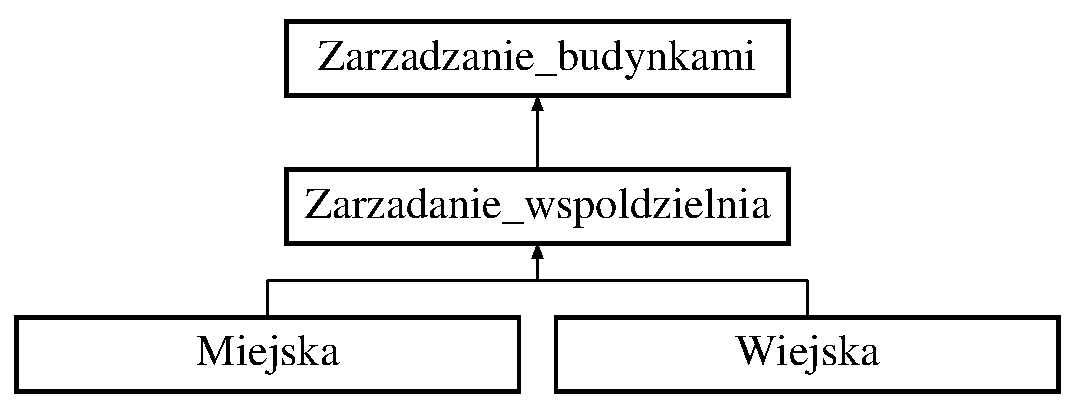
\includegraphics[height=3.000000cm]{class_zarzadzanie__budynkami}
\end{center}
\end{figure}
\subsection*{Public Member Functions}
\begin{DoxyCompactItemize}
\item 
\hypertarget{class_zarzadzanie__budynkami_ab0b3dbe88dc6ff684c15ec8438b51fc0}{}void \hyperlink{class_zarzadzanie__budynkami_ab0b3dbe88dc6ff684c15ec8438b51fc0}{info\+\_\+lista\+\_\+budynkow} ()\label{class_zarzadzanie__budynkami_ab0b3dbe88dc6ff684c15ec8438b51fc0}

\begin{DoxyCompactList}\small\item\em Funkcja wyswietlajaca informacje o budynkach. \end{DoxyCompactList}\item 
\hypertarget{class_zarzadzanie__budynkami_ab09c3e96b0877301050216f15affdd73}{}void \hyperlink{class_zarzadzanie__budynkami_ab09c3e96b0877301050216f15affdd73}{dodaj\+\_\+budynek} ()\label{class_zarzadzanie__budynkami_ab09c3e96b0877301050216f15affdd73}

\begin{DoxyCompactList}\small\item\em Funkcja umozliwiajaca dodanie budynku do spoldzielni. \end{DoxyCompactList}\item 
\hypertarget{class_zarzadzanie__budynkami_a20ae1255c7169fe8643f507cdab248a9}{}bool \hyperlink{class_zarzadzanie__budynkami_a20ae1255c7169fe8643f507cdab248a9}{usun\+\_\+budynek} ()\label{class_zarzadzanie__budynkami_a20ae1255c7169fe8643f507cdab248a9}

\begin{DoxyCompactList}\small\item\em Funkcja umozliwiajaca usuniecie budynku ze spoldzielni. \end{DoxyCompactList}\item 
\hypertarget{class_zarzadzanie__budynkami_aab94959cc237230127359a77aad3927f}{}virtual void \hyperlink{class_zarzadzanie__budynkami_aab94959cc237230127359a77aad3927f}{wczytaj\+\_\+z\+Pliku} ()=0\label{class_zarzadzanie__budynkami_aab94959cc237230127359a77aad3927f}

\begin{DoxyCompactList}\small\item\em Funkcja czysto wirtualna, umozliwiajaca wczytanie z pliku. \end{DoxyCompactList}\item 
\hypertarget{class_zarzadzanie__budynkami_a377271389f7fae1d2e99f31a7a9b2de1}{}virtual void \hyperlink{class_zarzadzanie__budynkami_a377271389f7fae1d2e99f31a7a9b2de1}{zapisz\+\_\+do\+Pliku} ()=0\label{class_zarzadzanie__budynkami_a377271389f7fae1d2e99f31a7a9b2de1}

\begin{DoxyCompactList}\small\item\em Funkcja czysto wirtualna, umozliwiajaca zapisanie do pliku. \end{DoxyCompactList}\item 
\hypertarget{class_zarzadzanie__budynkami_a323d1ac227348130b3f74ec3faa96cc3}{}virtual void \hyperlink{class_zarzadzanie__budynkami_a323d1ac227348130b3f74ec3faa96cc3}{info\+\_\+wspoldzielnia} ()=0\label{class_zarzadzanie__budynkami_a323d1ac227348130b3f74ec3faa96cc3}

\begin{DoxyCompactList}\small\item\em Funkcja wirtualna umozliwiajaca wyswieltlenie informacji o spoldzielni. \end{DoxyCompactList}\end{DoxyCompactItemize}
\subsection*{Protected Attributes}
\begin{DoxyCompactItemize}
\item 
vector$<$ \hyperlink{class_budynek}{Budynek} $>$ \hyperlink{class_zarzadzanie__budynkami_ae401202072085302f3d452a3279a2015}{budynki}
\end{DoxyCompactItemize}


\subsection{Detailed Description}
Klasa abstrakcyjna. 

\subsection{Member Data Documentation}
\hypertarget{class_zarzadzanie__budynkami_ae401202072085302f3d452a3279a2015}{}\index{Zarzadzanie\+\_\+budynkami@{Zarzadzanie\+\_\+budynkami}!budynki@{budynki}}
\index{budynki@{budynki}!Zarzadzanie\+\_\+budynkami@{Zarzadzanie\+\_\+budynkami}}
\subsubsection[{budynki}]{\setlength{\rightskip}{0pt plus 5cm}vector$<${\bf Budynek}$>$ Zarzadzanie\+\_\+budynkami\+::budynki\hspace{0.3cm}{\ttfamily [protected]}}\label{class_zarzadzanie__budynkami_ae401202072085302f3d452a3279a2015}

\begin{DoxyItemize}
\item Wektor budynkow spoldzielni. 
\end{DoxyItemize}

The documentation for this class was generated from the following file\+:\begin{DoxyCompactItemize}
\item 
/home/kamil/\+Pulpit/\+Elka/\+P\+R\+O\+E/\+P\+R\+O\+E-\/2/include/Zarzadzanie\+\_\+budynkami.\+h\end{DoxyCompactItemize}

%--- End generated contents ---

% Index
\backmatter
\newpage
\phantomsection
\clearemptydoublepage
\addcontentsline{toc}{chapter}{Index}
\printindex

\end{document}
